% SPDX-License-Identifier: CC-BY-4.0
% research-report.tex: 结题报告

% Authors: 吴骏东 <1904346407@qq.com>,
%          张子辰 <zichen350@gmail.com>,
%          蓝俊玮 <ljw13@mail.ustc.edu.cn>,
%          郭耸霄 <logname@mail.ustc.edu.cn> and
%          陈建绿 <2512674094@qq.com>

% Copyright (C) 2022 吴骏东, 张子辰, 蓝俊玮, 郭耸霄 and 陈建绿
% All rights reserved.

% 🅭 🅯
% This document is licensed under a Creative Commons Attribution
% 4.0 International license <https://creativecommons.org/licenses/by/4.0/>.
\documentclass{../runikraft-report}

\hypersetup
{
  pdftitle={2022春 操作系统原理与设计(H) x-runikraft小组 结题报告},
  pdfauthor={吴骏东; 张子辰; 蓝俊玮; 郭耸霄; 陈建绿}
}
\renewcommand{\today}{2022年7月9日}

\begin{document}
\title{\bfseries Runikraft小组\quad 结题报告\thanks{作者按Unicode码位排序,按贡献度排序是张子辰、郭耸霄、陈建绿、吴骏东、蓝俊玮。}}
\author{吴骏东\and 张子辰\and 蓝俊玮\and 郭耸霄\and 陈建绿}
\date{\today}
\maketitle

\tableofcontents

\section{项目简介}
Runikraft 是用Rust语言编写的能在RISC-V架构 + QEMU平台上运行的unikernel。
它基于用C语言实现的Unikraft,在继承Unikraft的高效性和可定制性的同时,
进一步简化了构建系统镜像的流程,加入了RISC-V支持,并且
用Rust语言提供了更强的内核安全保证。
与RustyHermit和rCore等用Rust实现的操作系统不同,
我们将完全使用Rust的稳定特性编写代码。

众所周知,在互联网技术和云计算不断发展的今天,我们身边的虚拟化设备不断增多,
它们中的很多都使用了Unikernel。然而,虚拟化设备和Unikernel也暴露出了很多安全问题。
对这些安全问题,C语言因其本身的缺陷难辞其咎。

Rust 是一门让人人都能写出可靠、高效的软件的语言。\cite{bib:feasibility-7}利用Rust编写Unikernel,
可以充分发挥它相对C语言的高层抽象和内存安全保证。用Rust改写项目已经成为一种解决问题的
有效手段,如zalando公司从Scala转向Rust的成功故事。\cite{bib:feasibility-3}

RISC-V是一款自由、开源的ISA,它开启了全新的基于开放标准协作的处理器创新时代。\cite{bib:feasibility-0}
目前基于RISC-V架构的开源处理器有很多,既有标量处理器Rocket,
也有超标量处理器BOOM,还有面向嵌入式领域的Z-scale、PicoRV32等。\cite{bib:feasibility-2}

因此,我们计划使用Rust语言改写架构和性能方面占优的unikernel——Unikraft。

\section{项目背景}
\subsection{操作系统的架构}
最初的操作系统缺乏明确定义的结构,也就是简单结构。这类系统的设计者希望用
最小的空间提供尽可能多的功能,因此,系统没有被仔细划分成模块,整个系统是
一个高度耦合的整体,用户程序的错误可能导致整个系统的崩溃。\cite{bib:os-concept}

随着操作系统的
发展,分层系统出现了,这种系统被分割成若干层,最低层为硬件层,最高层为用户
层,每一层都在较低层的基础上实现,并为较高层提供一组能调用的程序集。分层系统
简化了构建和调试系统的难度,并且有助于局部优化系统。
然而合理地定义各层并不容易,有时低层组件可能需要
高层组件提供的服务;而且分层会导致用户层执行的操作需要多次转发才能映射到硬件
操作,效率稍差。

随着分层系统的不断发展,系统的内核日益增大,这导致系统的内核愈发难以管理和维护。
微内核就是在这样的背景下诞生的,在这种系统中,只有CPU调度、内存管理、进程通信等
高度依赖特权的模块被放在内核中,而设备驱动、文件系统、网络等系统服务一概是运行
在用户态下的独立服务进程,这些服务进程依靠消息传递机制相互使用。微内核诞生后,原本
的分层系统的内核被称为宏内核。典型的微内核的
代码量在一万行以下,这有助于用形式化方法严格验证内核的正确性,确保内核没有安全漏洞
和功能缺陷。与此同时,运行在用户态下的服务进程之间相对独立,进程的权限恰能提供
相应的服务,一个进程的崩溃不会波及整个系统。所以,微内核系统相比宏内核更安全、
更健壮。虽然与宏内核相比,消息传递会降低系统模块之间的通信效率,但这可以通过共享内存缓解。

受微内核系统的启发,宏内核系统引入了可加载内核模块,即一项服务可以在系统启动后随时链入内核,
或从内核中卸载。
这样,内核的核心组件只需要包含CPU调度、内存管理、进程通信等基本的功能,而其他内核功能可以
根据需要启动。不过,与微内核不同,这些可加载内核模块运行在内核态,它们中的安全漏洞可以
威胁整个内核。\cite{bib:os-concept}

传统上,操作系统应该为用户程序提供尽可能全面的服务,并且要负责在用户程序和系统间、
用户程序之间建立屏障,以防止用户程序的错误影响整个系统。但是,随着计算机的普及,
专为一个用途建造的计算机愈来愈多,这些计算机上只会运行一个用户程序,而这个用户程序
的崩溃也意味着系统的崩溃,所以传统操作系统中的隔离在这种高度专用的计算机中毫无意义,
而消除隔离能减小上下文切换的开销,进而提高效率。当今,需要大量使用专用系统的领域
包括物联网、工业控制和云计算。前两者主要需要实时系统,而后一者与虚拟化密切相关。

\subsection{虚拟化}
在1960s,大型机的运算速度已经远超过了人类的操作速度。为了
充分利用大型机的算力,一台大型机配置了多个终端,多个用户可以同时通过终端与大型机交互,
多个用户的程序轮转使用CPU时间。由于轮转速度很快,用户无法感受到自己的程序没有连续运行,
所以在每个用户看来,他似乎拥有一台独立的计算机。这种运行在大型机上的分时系统是最初的虚拟化。
然而,随着个人计算机的发展,这种基于分时系统的虚拟化逐渐没落。虚拟化的再次兴起
得益于互联网技术的发展和云计算的兴起,在云计算中,用户通过网络操作远程的虚拟机,
这些远程虚拟机可以向外界提供网络服务。

\subsubsection{虚拟机}\sectionauthor{张子辰}
广义上的虚拟机是模拟硬件或解释高级语言的程序,比如Apple在两次macOS架构迁移时
分别推出的Rosetta和Rosetta 2就是硬件模拟器,CPython就是高级语言解释器,
而OpenJDK JRE可以视为硬件模拟器,只不过它模拟的是不存在的硬件。这三个示例
都侧重协助运行程序,而几乎没有隔离措施。狭义的虚拟机是一个模拟完整的计算机系统
的程序,在虚拟机上运行的系统看来,虚拟机和物理机没有明显区别,而且,虚拟机上
运行的系统不能随意访问宿主机的资源,Virtual Box、VMWare就是这类虚拟机。
由于云计算平台上运行的用户程序对计算资源的提供商并不可信,所以,提供商希望将用户
程序与系统的其他部分隔离。这需要狭义的虚拟机。

最初的云计算服务就是向用户提供一台完整的远程虚拟机。通常的远程虚拟机帮助用户提供
网络服务,也就是作为服务器。服务器其实不需要每时每刻都保持运行,而只需要在有人请求这项网络
服务时运行,但是为了确保网络服务的可用性,服务器必须保持开机,用户必须
持续为这台作为服务器的远程虚拟机付费。为了更细粒度地分配计算资源,云计算服务的提供商
推出了serverless服务。在serverless中,原本的服务器被拆分成若干“函数”,其实也就是
一个响应网络请求的程序。当网络服务被请求时,这个程序被启动,响应这个请求,然后退出。
这需要一台虚拟机能够快速启动,可是传统的虚拟机无法满足要求。

\subsubsection{容器}\sectionauthor{蓝俊玮}
一种解决方案是不使用虚拟机,而使用更加轻量的方式实现隔离,比如容器。
以Docker为代表的传统容器是为了便捷地打包程序及其依赖诞生的,而并不强调隔离性。
传统容器使用 Namespace/Cgroup 实现,这套容器技术实际上是从进程调度的角度入手,
对内核进行的功能扩展。优势上来说,操作界面很 Linux、很方便,开销也很低,
可以被用来无负担地套在已有应用外面,来构建隔离的环境。并且它是纯软件方案,
不和其他层面的物理机、虚拟机相冲突。然而,
随着容器技术的不断发展,传统容器隔离性不足的缺陷逐渐暴露了出来。
Namespace/Cgroup 是内核的一个部分,其中运行的容器仍然使用主机的 Linux 内核,
它解决不了Linux内核中隔离性差的问题,攻击者可以利用Linux内核的漏洞
实现容器逃逸,然后便可以直接对宿主机进行攻击。\cite{bib:docker-security-selinux}

基于操作系统本身的容器机制没办法解决安全性问题,需要一个隔离层。
而虚拟机是一个现成的隔离层,AWS这样的云服务已经让全世界相信,
对用户来说,“secure of VM” 是可以满足需求的。
虚拟机里面只要有个内核,就可以支持 OCI 规范的语义,
在内核上跑个 Linux 应用并不太难实现。所以,安全容器的隔离层让应用的
问题——不论是恶意攻击,还是意外错误——都不至于影响宿主机,
也不会在不同的 Pod 之间相互影响。而且实际上,额外隔离层带来的影响并不仅是安全,
对于调度、服务质量和应用信息的保护都有好处。目前的安全容器有两个主流实现:
\begin{itemize}
\item \href{https://github.com/kata-containers/kata-containers}{Kata Container} 是MicroVM的一个经典的实现,它提供了一个MicroVM,
并且有专门提供给 Kubernetes 的接口,有比较好的安全性和运行效率,
现在已经开始逐步使用。但是其启动时间和内存占用与传统容器还有一定的差距。
\item  \href{https://github.com/google/gvisor}{gVisor} 是
基于进程虚拟化的容器实现,它拥有很好的隔离性,
很小的内存占用和启动时间,但是系统调用效率不高。
\end{itemize}

容器虽然解决了传统虚拟机启动时间长的问题,但是无法兼顾效率和隔离性。

\subsubsection{Unikernel}\sectionauthor{张子辰 and 陈建绿}
Unikernel在MicroVM的基础上更进一步,它放弃了运行在虚拟机上的系统内的隔离,让用户程序
和系统程序运行在同一个地址空间下,用户通过函数调用(如\texttt{call}指令)
而不是软中断或陷入(如\texttt{int}、\texttt{syscall}、\texttt{ecall}等指令)使用
系统提供的服务,这免去了上下文切换的开销,大幅提高了系统调用的效率。
高效的系统调用甚至使unikernel的响应时间和吞吐率优于容器。
由于unikernel本质上是运行在虚拟上
的独立操作系统,它拥有良好的隔离性。Unikernel的系统镜像中只包含了用户程序
需要的代码,这使unikernel的镜像非常轻量,甚至比Docker镜像还小。

然而,为了追求轻量性,
unikernels裁剪了传统的操作系统的众多组件,因此unikernels无法提供许多
常用的库的应用程序接口,所以为了将现有的程序移植到某个unikernel平台,开发者
不得不根据该unikernel的API重构程序。\cite{bib:unikraft}
此外,为了轻量、快速,unikernels
没有启用许多基本的并且不会影响性能的安全措施,这导致unikernels相比容器
更容易受到用户程序的安全漏洞的影响。\cite{bib:unikernel-secuirty}

目前的Unikernel 按实现方式大致可以分为两种:
\begin{itemize}
\item 全新的方式(Clean-slate):在构建单一用途的操作系统的假设下,
自由地使用现代工具来进行构建,比如模块化(modularity)、
声明性代码(declarative code)、避开样板文件(avoiding boilerplate)等。
并且从头开始思考操作系统和应用程序层的实现,
使用高级语言进行系统库的编写,从而使得实现更加可掌控,得到的系统库质量更高。
用 OCmal 语言编写的 MirageOS 就是使用 Clean-slate 方式实现的。
\item 传统的方式(Legacy):在不进行修改或只进行一些小的修改的前提下,
运行现有的软件。这通常通过将现有的操作系统代码库重构到库操作系统中来实现。
用 C 语言编写的 Rumprun 是使用 Legacy 方式实现的。
\end{itemize}

\subsection{Unikernels面临的问题}
Unikernel是为了解决容器的隔离性差和传统的虚拟机启动慢而诞生的,所以unikernels
必须做到启动快、延迟低、吞吐量大。Unikernels的目标是取代容器,成为云计算领域的
最佳选择,所以它们必须提供高效的网络支持。为了方便现有的程序移植到unikernels上,
unikernel应该考虑兼容性问题,它们应该以最小的代价提供目前常用的系统APIs,并且
移植目前常用的库。此外,unikernels镜像的构建不应该过于繁琐。

\subsection{知名的Unikernels}\label{subsec:famous-unikernel-projects}
下面简要介绍我们详细调研了的七个近两年仍然在维护的unikernels。

\subsubsection{ClickOS}\sectionauthor{蓝俊玮}

ClickOS 是一个基于 Xen 的高性能的虚拟化软件中间盒平台。为了达到高性能,
ClickOS 对 Xen 的 I/O 子系统实现了广泛的翻修,包括对后端交换机、
虚拟网络设备和后端前端驱动程序。这些更改使 ClickOS 能够显著加快中间盒运行时的网络连接。\cite{bib:12-clickos}

ClickOS 虚拟机只有5MiB ,启动仅需要大约30ms,而且延迟只有45µs。
ClickOS 实现了广泛的中间盒,包括防火墙、运营商级 NAT 和
负载均衡器,并证明 ClickOS 可以每秒处理数百万个数据包,达到生产级性能。\cite{bib:12-clickos}\cite{bib:13-clickos2}

\begin{figure}[!hbt]
\begin{minipage}{0.49\linewidth}
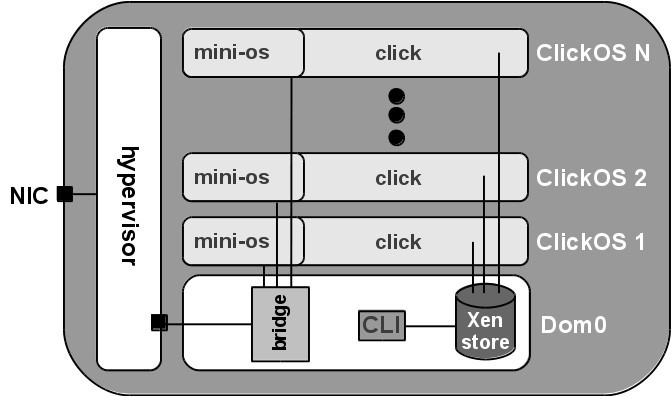
\includegraphics[width=\linewidth]{assets/clickOS_arch.jpg}
\caption{ClickOS 的架构\cite{bib:13-clickos2}}
\end{minipage}
\begin{minipage}{0.49\linewidth}
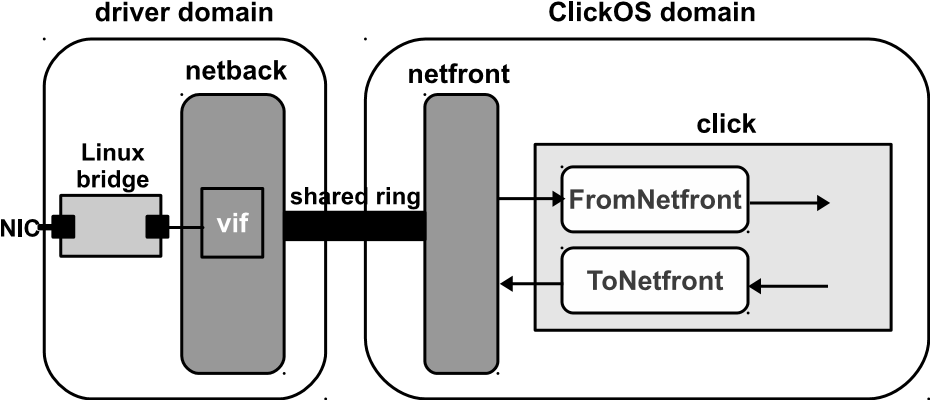
\includegraphics[width=\linewidth]{assets/ClickOS_networking.png}
\caption{Basic ClickOS networking in Xen\cite{bib:12-clickos}}
\end{minipage}
\end{figure}

\subsubsection{MirageOS}\sectionauthor{蓝俊玮}

MirageOS 是一个用 OCaml 语言编写的,
用于在各种云计算和移动平台构建安全、高性能的网络应用程序的库操作系统。
它可以将大型服务器划分为很多更小的虚拟机,使得服务器具有更强的拓展性和安全性。
其代码可以在 Linux 、Mac OS 等系统中开发,然后编译成一个完全独立的、专门的内核,
可以在 Xen、KVM hypervisors 或轻量级 hypervisors 下运行。MirageOS
已经发展成为一个由近100个开放源码库组成的成熟库,实现了一系列广泛的功能,
并且正开始与 Citrix XenServer 等商业产品集成。MirageOS
将 Xen hypervisors当成一个稳定的硬件平台,让我们可以专注于实施高性能协议,
没必要为支持传统操作系统里面的成千上万个设备驱动程序而操心。\cite{bib:11-unikerel2}

\begin{figure}[!hbt]
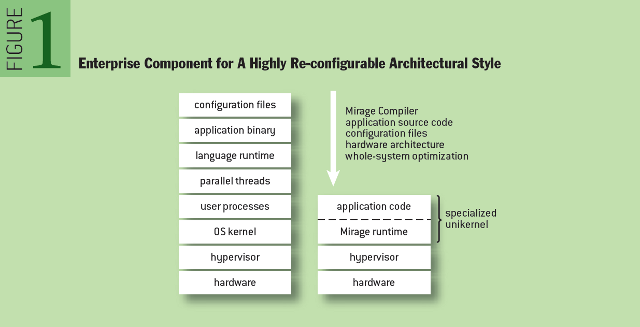
\includegraphics[width=\linewidth]{assets/figure1.png}
\caption{MirageOS 的架构}\label{fig:mirage-fig1}
\end{figure}

\begin{figure}[!hbt]
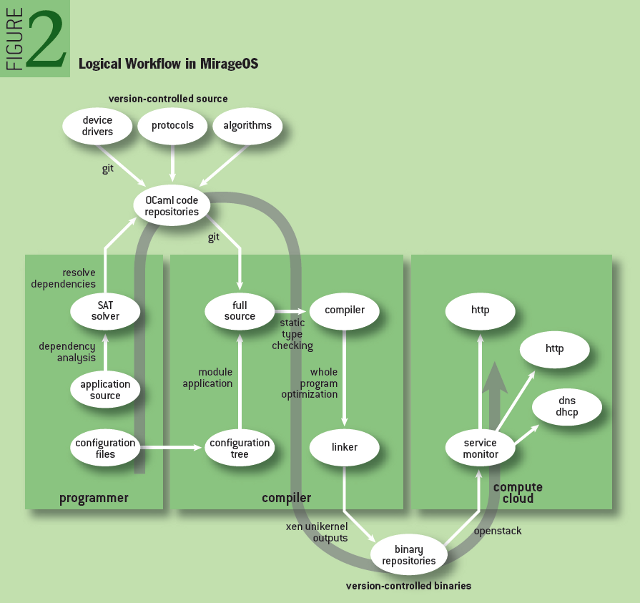
\includegraphics[width=\linewidth]{assets/figure2.png}
\caption{MirageOS的逻辑工作流}\label{fig:mirage-fig2}
\end{figure}

MirageOS的亮点是输入应用程序的所有源代码依赖项都被显式跟踪,包括实现内
核功能所需的所有库。MirageOS 包括一个构建系统,该系统内部使用
一个 SAT 解算器(使用 OPAM 包管理器,使用 Mancoosi 项目的解算器)
从一个已发布的在线包集中搜索兼容的模块实现。得益于 OCaml 的静态类型
检查,在编译时将捕获接口中的任何不匹配。

在 MirageOS 中,OCaml 编译器接收整个内核代码的源代码,
并将其链接到一个独立的本机代码对象文件。它链接到提供引导支持和
垃圾回收器的最小运行时。没有抢占式线程,内核是通过一个 I/O 循环轮询
Xen 设备的事件驱动的。\cite{bib:11-unikerel2}

\subsubsection{IncludeOS}\sectionauthor{蓝俊玮}

IncludeOS 是一个为开发基于 unikernel 的应用程序而创建 C++ API 的项目。\cite{bib:9-includeos}

当 IncludeOS 映像引导时,它通过设置内存、运行全局构造函数、注册驱动程序和中断处理
程序来初始化操作系统。IncludeOS 不支持虚拟内存,应用程序和
unikernel 库使用单个地址空间。因此,没有系统调用或用户空间的概念; 所有操作系统服务
都通过对库函数的简单调用使用,并且都以特权模式运行。\cite{bib:10-includeos2}

\noindent IncludeOS 有如下优点:\cite{bib:9-includeos}
\begin{itemize}
\item IncludeOS中目前没有进程抢占,所以操作系统的行为非常静态。
只要机器本身是可预测的,延迟也将是完全可预测的。因此,在裸机硬件上,
IncludeOS可被视为低延迟,可预测的操作系统。
\item 对网络的支持很好,与 Linux 相比表现出色。
\item IncludeOS 系统作为一个整体进行编译和优化。在编译和连接阶段,
优化器可以更多地了解整个系统正在做什么,并且有可能进一步优化。
\item IncludeOS 中的所有 IRQ 处理程序简单地(原子地)更新计数器,
并在有时间时将进一步的处理推迟到主事件循环。这消除了对上下文切换的需要,
同时也消除了与并发相关的问题,如竞争条件。
IncludeOS的所有 I/O 都是异步的,CPU 保持忙碌,不会发生阻塞。
\end{itemize}

\noindent IncludeOS 有如下缺点:\cite{bib:9-includeos}
\begin{itemize}
\item IncludeOS 不实现所有 POSIX。开发人员认为,
只有在需要时才会实现 POSIX 的某些部分。开发人员不太可能将完全遵守 POSIX 作为一个目标。
\item 与MirageOS一样,IncludeOS 中没有实现阻塞调用,因为当前的事件循环模型是使用它的最佳方式。
\item IncludeOS 目前还缺少可写的文件系统。
\end{itemize}

\subsubsection{RustyHermit}\sectionauthor{陈建绿}

\href{https://github.com/hermitcore/rusty-hermit}{RustyHermit}\ 是
一个基于 Rust 的、轻量级的 Unikernel,也是一个用来评估操作系统新的设计的研究项目。
它用 Rust 语言完全改写了 RWTH Aachen University
开发的研究项目 \href{http://hermitcore.org/}{HermitCore}\footnote{HermitCore 最初是用 C 语言编写的,
是一种针对高性能和云计算的可伸缩和可预测的运行时的 Unikernel。}。\cite{bib:14-rusty-hermit}

该项目完全使用 Rust 语言开发,Rust 的所有权模型保证了它的内存/线程安全,
并且让开发者能够在编译时就消除许多种 bugs。因此,与通用编程语言相比,使用 Rust
进行内核开发会留下更少的漏洞,得到更加安全的内核。

开发者扩展了 Rust 工具链以至于 RustyHermit 的 build 过程
与 Rust 通常的工作流程相似。使用 Rust runtime 而且不直接使用 OS 服务的
Rust 应用程序能够直接在 RustyHermit 上运行而不需要修改。因此,原则上,
每一个现有的 Rust 应用程序都可以建立在 RustyHermit 之上。\cite{bib:17-rusty-hermit2}


RustyHermit 中优化实现了网络栈。它使用 \href{https://github.com/smoltcp-rs/smoltcp}{smoltcp}
作为它的网络栈,使用 \href{https://www.linux-kvm.org/page/Virtio}{Virtio}
作为客户机和主机操作系统之间的接口。

Sung, Olivier, Lankes and Ravindran\cite{bib:18-intra-unikernel}
提出了一个修改版本的 RustyHermit,该版本利用Intel MPK(Memory Protection Keys)\cite{bib:19-mpk},
在保持单一地址空间的同时,在 Unikernel 实例中引入内存隔离,
包括安全内核代码与不安全内核代码之间的隔离、内核代码与用户代码之间的隔离。
在一组宏基准测试中,带有隔离功能的 unikernel 仅减慢了0.6\%。

\subsubsection{Rumprun}\sectionauthor{陈建绿}

Rumprun unikernel 是在 rump kernels 的基础上开发的。
Rumprun 不仅可以在像 KVM 和 Xen 这样的管理程序上工作,
还可以在裸金属上工作。无论有没有 POSIX-y 接口,Rumprun 都
可以正常使用。如果有 POSIX-y 接口,Rumprun 则允许现有的、
未经修改的 POSIX 应用程序开箱即用;如果没有 POSIX-y 接口,
Rumprun 则允许构建高度自定义的解决方案,并且占用的空间最小。

Rumprun unikernel 支持用 C、 C++ 、 Erlang、 Go、
Java、 Javascript (node.js)、 Python、 Ruby 和 Rust 等语言编写的应用程序。

在\ \href{https://github.com/rumpkernel/rumprun-packages}{rumprun-packages repository}\
中可以找到用于 Rumprun 的现成软件包,比如 \texttt{LevelDB},
\texttt{Memcached}, \texttt{nanomsg}, \texttt{Nginx} 和 \texttt{Redis}。

\paragraph{1. Rump kernels}~

Rump kernels 的组件来自未经修改的 NetBSD,由此开发者提供了一个 POSIX-y API。
Rump Kernel 项目以一种可用于构建轻量级、特殊用途虚拟机的形式提供了 NetBSD 的
模块化驱动程序。因为开发者没有做会将错误引入到应用程序运行时(application runtime)、
libc 或驱动程序中的移植工作,所以程序可以很稳定地工作。\cite{bib:21-rump-kernel}
\begin{figure}[!hbt]
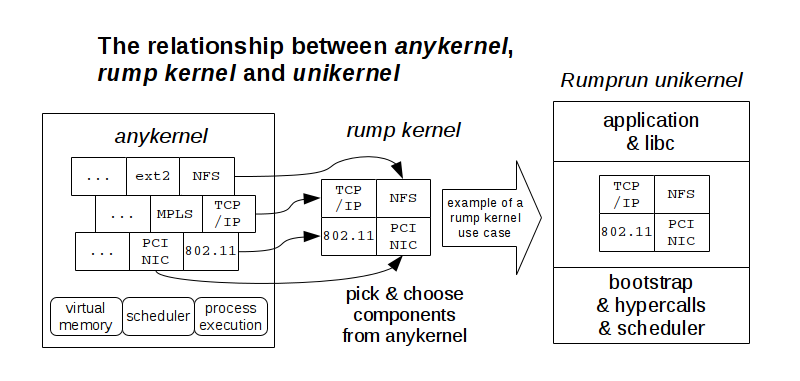
\includegraphics[width=\linewidth]{assets/rumprun-1.png}
\caption{Anykernel、
Rump kernel 和 Rumprun Unikernel 的关系}
\end{figure}

\begin{quote}
“Anykernel”概念指的是一种与架构无关的驱动程序方法,在这种方法中,驱动程序既可以编译到宏内核中,也可以作为用户空间进程运行,具有微内核风格,并且不需要修改代码。\\
\hspace*{\fill}——维基百科
\end{quote}

\paragraph{2. Rumprun}~

Rumprun 可用于将几乎任何与 POSIX 兼容的程序转换为一个可工作的
Unikernel。使用 Rumprun,理论上可以将 Linux 或者 类Unix系统上的大部分
程序编译成 Unikernel。Rumprun 以开发 NetBSD 内核中的驱动程序并在用户空间
中进行测试的需求为出发点,主要的工作是重构这个代码库,使其看起来像一个库操作系统。\cite{bib:24-rumrun}

\begin{figure}[!hbt]
\begin{minipage}{0.49\linewidth}
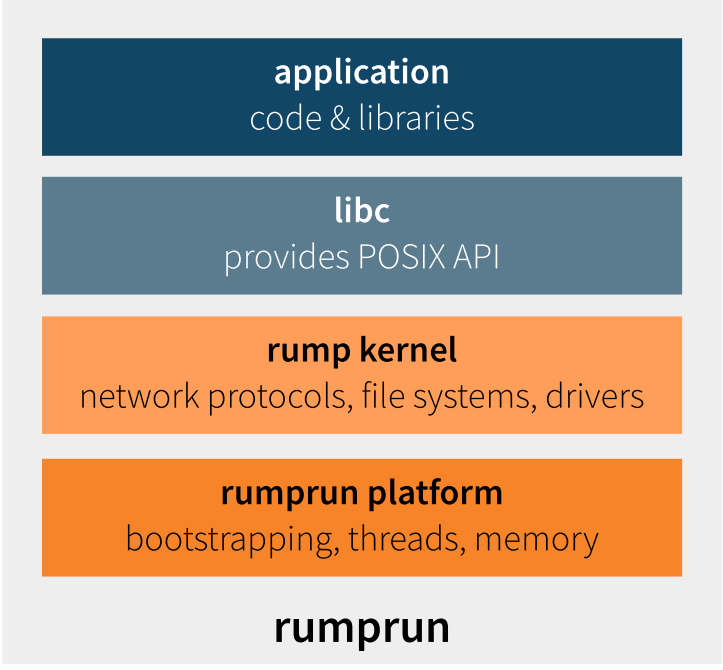
\includegraphics[width=\linewidth]{assets/rumprun-2-cut.png}
\caption{Rumprun 的架构}
\end{minipage}
\begin{minipage}{0.49\linewidth}
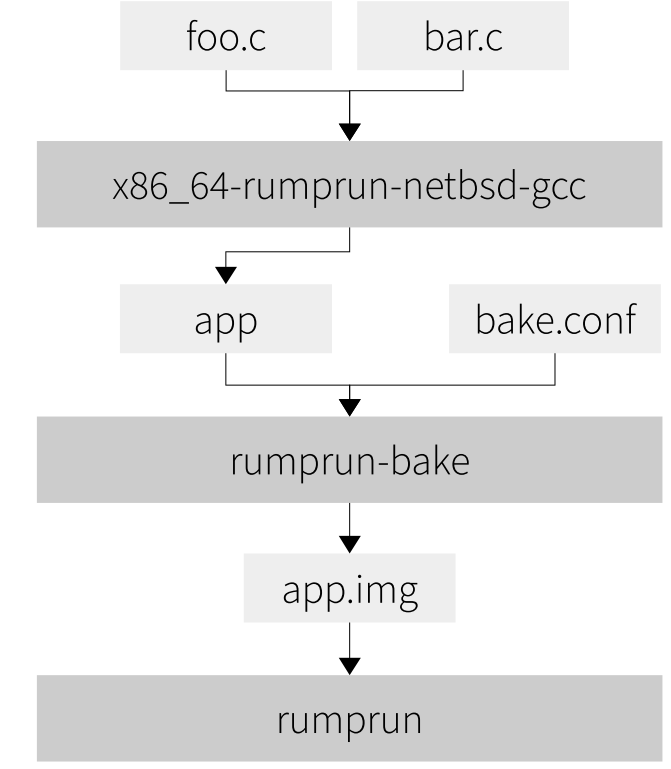
\includegraphics[width=\linewidth]{assets/rumprun-3-cut.png}
\caption{Rumprun 的工作流程示例}
\end{minipage}
\end{figure}

Rumprun 也有一些限制:

\begin{itemize}
\item single address-space
    \begin{itemize}
    \item no processes
    \item no virtual memory
    \item no signals
    \end{itemize}
\item toolchain
    \begin{itemize}
    \item still experimental
    \end{itemize}
\item threading
    \begin{itemize}
    \item cooperative
    \item single-core
        \begin{itemize}
        \item need to spawn multiple unikernels to use multiple cores
        \end{itemize}
    \end{itemize}
\end{itemize}

我在调研的过程中发现,rump kernel 的好多官方文档都会重定向到
\url{https://rumpkernel.org}这个网址,而这个网址目前只有一些 IT News,
并非和 rump kernel 相关的内容,所以猜测该项目目前已经无人维护。

\subsubsection{Nanos}\sectionauthor{陈建绿}

\href{https://github.com/nanovms/nanos}{Nanos}\ 一个比较新的正在开发中的 Unikernel。

\begin{itemize}
\item Nanos 是一个新的内核,旨在在虚拟化环境中运行一个且仅有一个应用程序。
与 Windows 或 Linux 等通用操作系统相比,它有几个限制——即它是一个单进程系统,
不支持运行多个程序,也不具备通过 ssh 进行用户或远程管理的概念。
\item Nanos 的目标是成为一个比 Linux 安全得多的系统。
它做到这一点的几个依赖:没有用户的概念,每个虚拟机只运行一个进程,限制每个虚拟机中包含的代码数量。
\item Nanos 并不打算在裸金属上运行,所以开发者努力使其内核尽可能简单。
\end{itemize}

\subsubsection{Unikraft}\sectionauthor{张子辰}
Unikraft是一个比较新的unikernel。它在设计时就充分考虑
了现有的unikernels的优缺点。它在保持unikernel的极简化、
高效的同时,引入了完整的POSIX兼容层,使开发者可以轻松地将现有的为Linux
编写的代码移植到unikernel上。Unikraft由若干低耦合的模块组成,内存分配器、
调度器、网络栈、引导代码都是独立的微型库。Unikraft的API即为微型库本身,
这意味着可以在生成时轻松地添加或移除APIs。\cite{bib:unikraft}

Unikraft遵从如下设计原则:
\begin{itemize}
\item 内核应该是完全模块化的,以便允许unikernel被彻底而轻松的定制。
在Unikraft中,内存分配器、调度器、网络栈、引导程序等系统原件都是
独立的微型库。
\item 内核应该提供注重效率、良定义的API,而且允许用户轻松地
为了满足自己的程序的性能要求选择、组装它们。在Unikraft中,这些APIs
就是微型库本身,这意味着它们可以轻松地在构建时增减,而且提供更多
的微型库即可拓展它们功能。
\end{itemize}

目前,Unikraft已经支持SQLite, nginx, Redis等程序,C/C++, Go, Python, Ruby,
Web Assembly and Lua等编程语言或运行环境。

在架构方面,Unikraft融合了宏内核的单地址空间带来的高效性和微内核的模块化带来的
可拓展性。OS的功能被分割成若干细粒子度的组件,而各个组件之间通过良定义的APIs
通信。Unikraft用精心设计的APIs和静态链接获得高效率,而不是为了效率破坏API
的边界。Unikraft大致分为两部分:
\begin{description}
\item[微型库]微型库是实现一部分的Unikraft的APIs的软件组件,
Unikraft的作者有意将它们分割到了不同的库中,并尽可能降低它们之间的依赖。
实现相同APIs的微型库可以相互替换。比如,Unikraft内核就提供了多种实现
\texttt{ukalloc}接口的内存分配器。
\item[构建系统]它为用户提供基于Kconfig的配置菜单\footnote{在实验1中,
我们在定制Linux内核时,运行\texttt{make menuconfig}后看到的就是Kconfig菜单。},
用户可用它选择要用哪些微型库,要为哪个平台和哪个CPU架构构建。
\end{description}
\begin{figure}[!hbt]
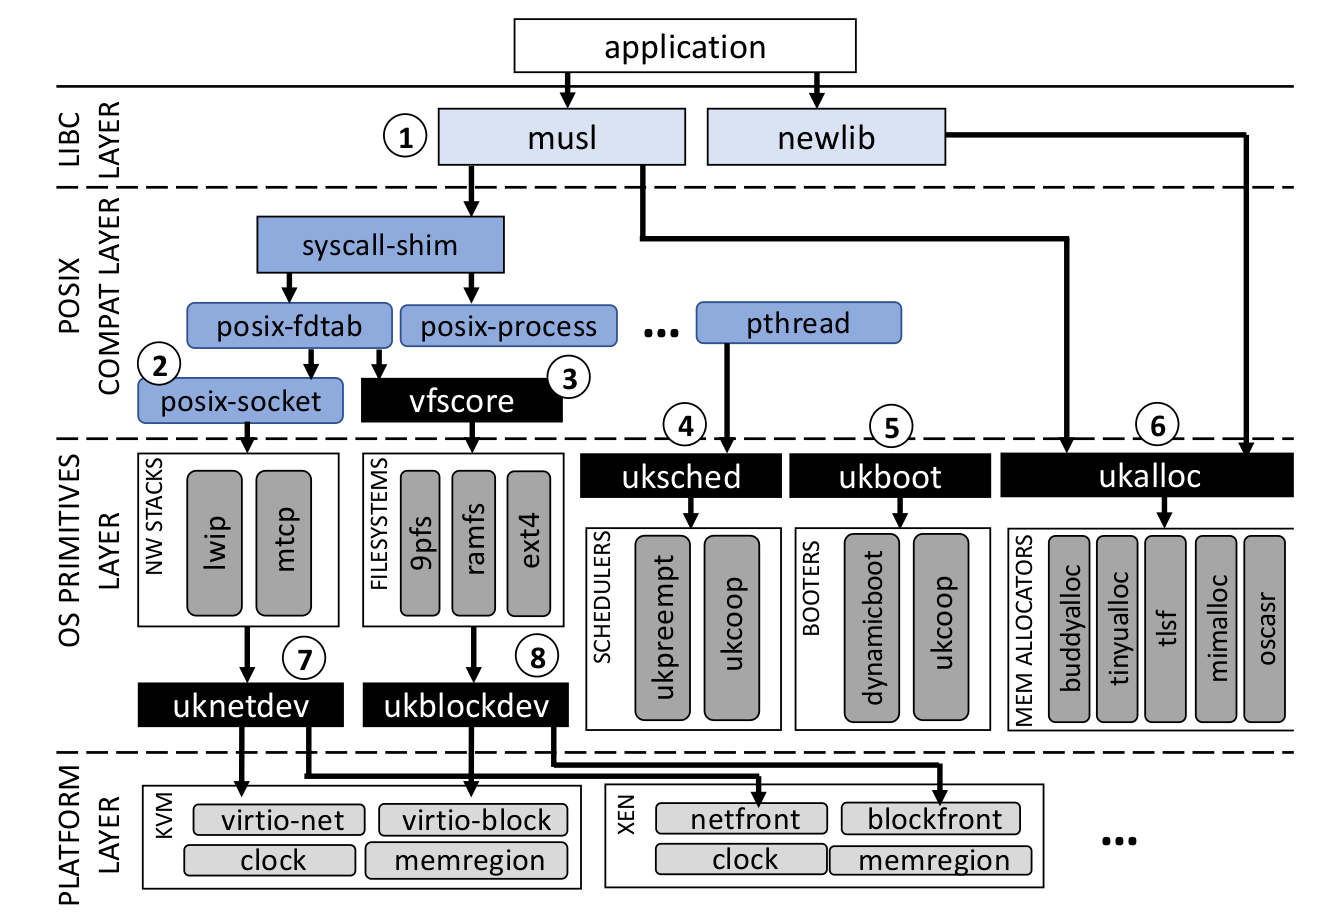
\includegraphics[width=\linewidth]{assets/Unikraft-architecture.png}
\caption{Unikraft的架构(黑色框内的是APIs)允许用户程序接入不同层次的APIs,也
允许用户选择不同的API实现。}\label{fig:unikraft-arch}
\end{figure}

图\ \ref{fig:unikraft-arch}\ 展示了Unikraft的架构。使用不同层次的APIs和
替换API实现的能力给开发者提供了多种优化可能。首先,未经修改的程序(如用C语言
写的Hello World和nginx)可以使用\texttt{musl}(图\ \ref{fig:unikraft-arch}\ 的①)
或\texttt{nolibc}提供的POSIX兼容层,并自动获得低启动时间、低内存消耗和
更高的吞吐量,因为在Unikraft中,系统调用是高效的函数调用。

类似地,程序的开发者可以轻松选择合适的内存分配器(⑥)以达到最高效率,甚至
在同一个unikernel中使用多种分配器。

关注快速引导的开发者也可以使用自己的遵守\texttt{ukboot} API的引导代码(⑤)。
对于网络密集型程序,开发者可以使用标准的套接字接口(②),或者使用更底层、更高效
的\texttt{uknetdev} API(⑦)以便大幅提高吞吐量。

类似地,数据库这样的硬盘密集型程序可以使用标准的\texttt{vfscore}微型库(③),
或者用\texttt{ukblock} API提高吞吐量(⑧)。

调度器也是可插拔的(④),而且每个CPU核可以运行不同的调度器。


与其他unikernels相比,Unikraft的系统镜像更小、运行所需内存更小、吞吐量更大:
\begin{figure}[H]
\centering
\begin{minipage}{0.32\linewidth}
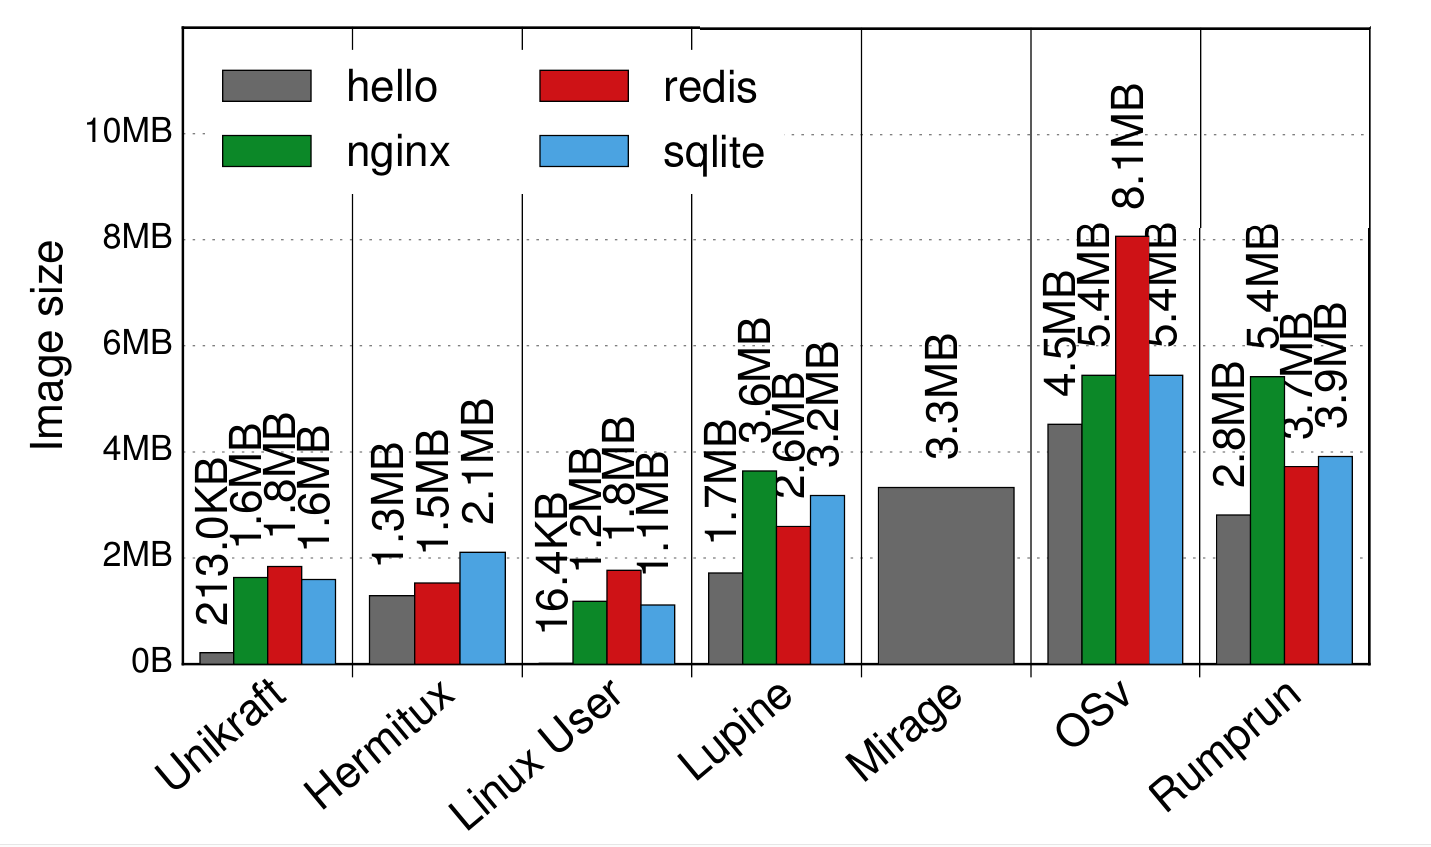
\includegraphics[width=1\linewidth]{assets/Unikraft-image-size.png}
\caption{}
\label{fig:unikraft-image-size}
\end{minipage}
\begin{minipage}{0.32\linewidth}
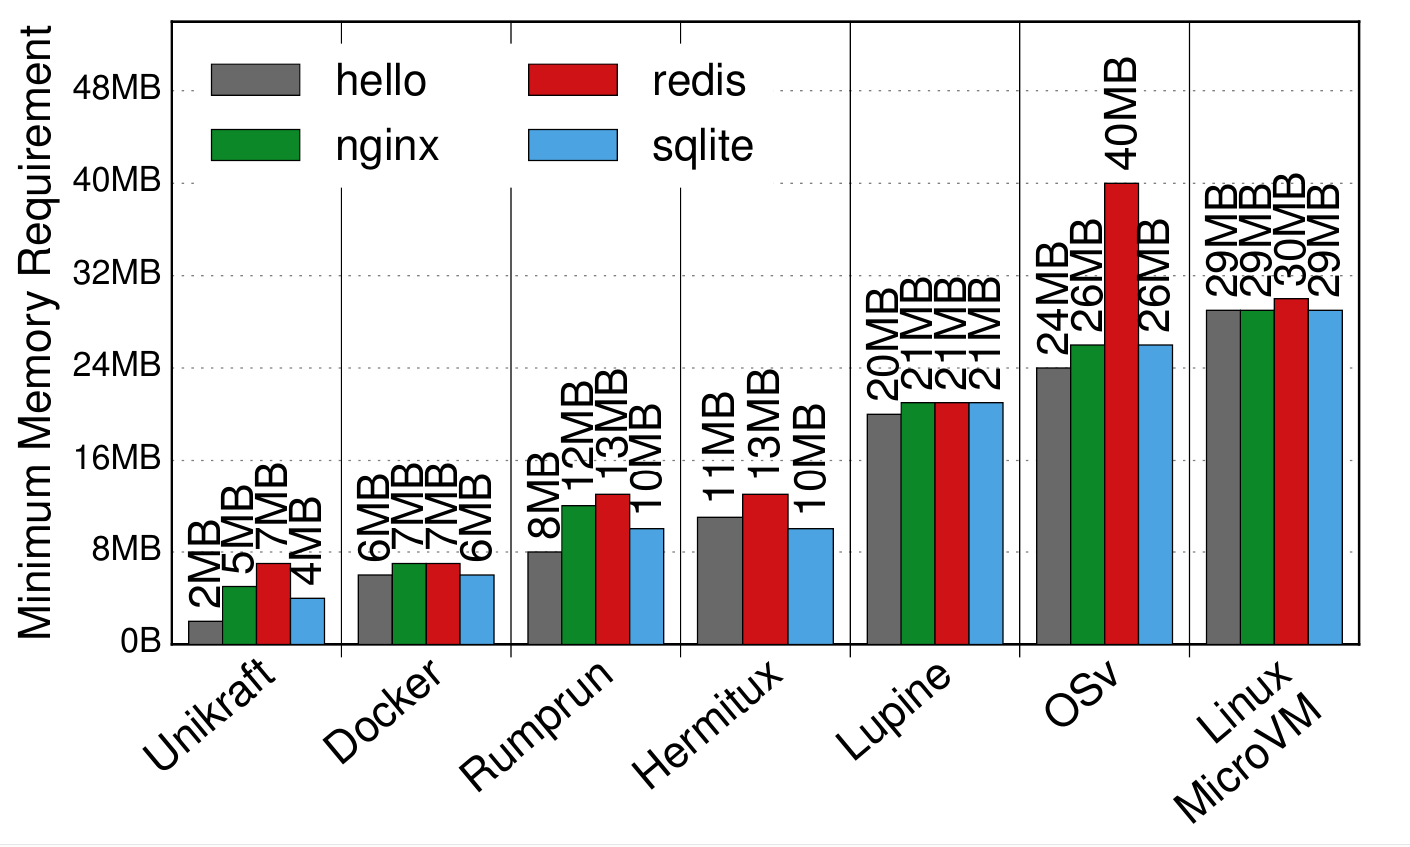
\includegraphics[width=1\linewidth]{assets/Unikraft-memory.png}
\caption{}
\end{minipage}
\begin{minipage}{0.32\linewidth}
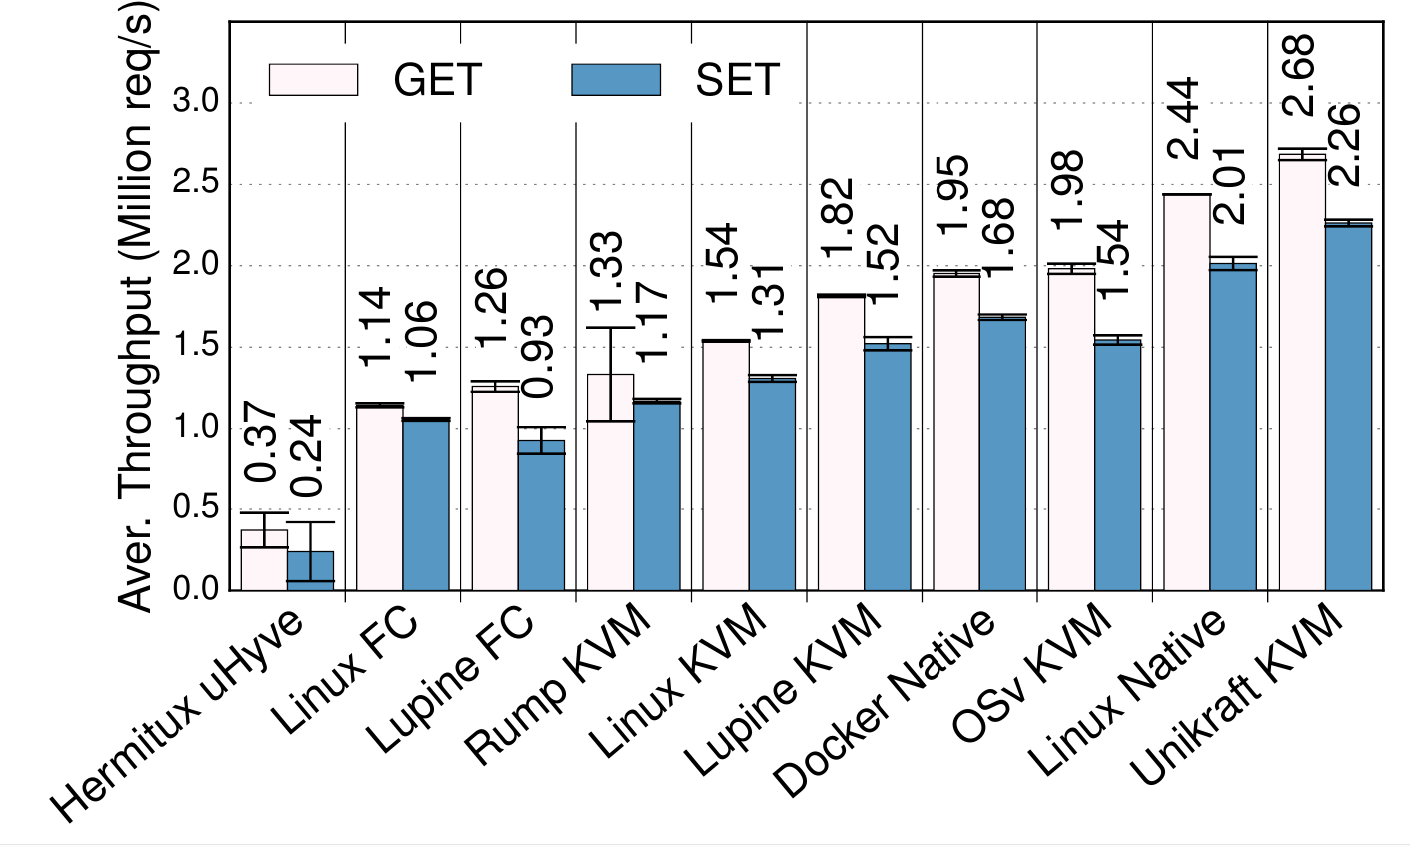
\includegraphics[width=1\linewidth]{assets/Unikraft-throughput.png}
\caption{}
\end{minipage}
\end{figure}

Unikraft在提升效率的同时兼顾了安全性。根据NCC Group\cite{bib:unikernel-secuirty},
虽然 unikernel 相比容器体积更小、隔离性更好,但是由于不存在内核态-用户态隔离,
且缺乏W\^{}X、stack canary等安全特性,unikernel 其实比传统的容器更不安全。
也就是说,攻击者可以利用 unikernel 上的程序的漏洞,控制 unikernel 所在的虚拟机,
进而未经授权访问资源。

所以,不能片面地把安全性与隔离性等同。而且我们不能
片面地认为使用 Rust 这样的安全的程序设计语言就能保证安全,
因为完整的 unikernel 上不只包含安全的系统代码(或者说库代码),还包含可能不安全的用户代码,
而后者可以导致整个系统不安全。因此,要实现安全的 unikernel,不能仅仅依靠安全的程序设计语言,
而需要额外的安全特性。

NCC Group提到了ASLR、分页保护(如W\^{}X政策、内部数据加固、保护页、空页面漏洞等)、
栈保护标志\footnote{它的英文stack canary来自金丝雀曾经被用来检查煤矿的有毒气体的典故\cite{bib:canary}。}、堆加固、标准库加固等安全措施。

它测试了 rumprun 和 includeOS 两个 unikernels,并发现它们几乎没有实现任何安全特性。

尽管 Unikraft 使用 C 语言实现,但它支持(或计划支持)
\href{https://github.com/unikraft/unikraft/tree/staging/lib/uksp}{Stack SP}、
\href{https://github.com/unikraft/unikraft/tree/staging/lib/ubsan}{UBSAN}、
\href{https://github.com/unikraft/unikraft/pull/421}{ARM BTI}、\href{https://github.com/unikraft/unikraft/pull/191}{KASAN}、\href{https://github.com/unikraft/unikraft/pull/239}{PIE}、True Random Number Generator、
Intel CET、ARM SB等安全特性。\cite{bib:unikraft-secuirty}

\subsubsection{比较}\sectionauthor{张子辰}
表\ \ref{table:unikernel-compare}\ 比较了我们详细调研的unikernels。因为现有的
资料并没有包含我们需要的所有信息,表中的一些信息是依靠阅读源代码获取的。
\small
\begin{longtable}{|c*{7}{|>{\centering\arraybackslash}p{0.095\linewidth}}|}
\caption{Unikernels的比较}\label{table:unikernel-compare}\\
\hline
&ClickOS&\resizebox{\linewidth}{\height}{MirageOS}&\resizebox{\linewidth}{\height}{IncludeOS}&\resizebox{\linewidth}{\height}{RustyHermit}&Nanos&Rumprun&Unikraft\\\hline
\endfirsthead
\hline
&ClickOS&\resizebox{\linewidth}{\height}{MirageOS}&\resizebox{\linewidth}{\height}{IncludeOS}&\resizebox{\linewidth}{\height}{RustyHermit}&Nanos&Rumprun&Unikraft\\\hline
\endhead
实现语言&C++&OCaml&C++&Rust&C&C&C\\\hline
支持架构&x86-32、x86-64&x86-64、ARM-64&x86-32、x86-64、ARM-64&x86-64、ARM-64&x86-64、ARM-64、RISCV-64&x86-32、x86-64、ARM-64&x86-64、ARM-32、ARM-64\\\hline
支持平台&Xen&KVM、Xen&KVM、Virtual Box、VMWare、x86物理机&QEMU、Uhyve&众多,包括但不限于Xen、KVM、VMWare、Virtual Box等&Xen、嵌入式设备&KVM、Xen、Solo5、Linux用户态\\\hline
支持语言&C、C++&OCaml&C、C++&Rust、C、C++、Go、Fortran&众多,包括但不限于C、Go、PHP、Node、Ruby、Lua、Perl等,理论上支持任何ELF文件&众多,包括但不限于C、C++、Erlang、Go、Java、Javascript (node.js)、Python、Ruby 、Rust等&众多,包括但不限于C、C++、Go、Python、Ruby、Web Assembly、Lua等\\\hline
构建系统&Click configuration language&Opam&Conan、CMake&cargo、CMake&系统与用户程序分别构建,系统使用Makefile构建&buildrump&Kraft、Kconfig\\\hline
安全性&不详&用安全语言实现,支持random device&较差,甚至关闭了一些C++编译器支持的安全特性&
用安全语言实现,支持堆栈保护、应用程序堆栈与操作系统库堆栈分离,有支持页保护的衍生作品&支持ASLR、页保护&有限,\texttt{.text}段不可写,有一定的堆保护,默认引入大量无用库&支持Stack SP、UBSAN、ARM BTI、PIE、Intel CET、random device等安全特性\\\hline
API&专用API&OCaml标准库,和大量其他用OCaml实现的库&不完整的C、C++、POSIX API支持&Rust标准库,部分C、C++、Go、Fortran API&无,依靠系统调用与用户程序通信&C、POSIX API和大量软件包,默认开启系统调用&专用API、POSIX API、C API和众多库\\\hline
网络&有&有&有&用smoltcp实现&有&有&可选择lwip和mtcp两种实现\\\hline
内存管理&有&有,支持垃圾回收&有&有&有&有&有,可以选择多种分配器\\\hline
线程管理&有&无抢占,有进程通信支持&有&有,支持优先级&有&无抢占&支持抢占和无抢占两种调度器,有进程通信支持\\\hline
文件管理&无&支持FAT和mmap&支持mmap和读FAT32&可以支持多种文件系统后端,目前支持virtio-fs和mmap&有&有&支持9pfs和mmap\\\hline
备注&基于MiniOS&&&&相比unikernel,Nanos更像一个微型内核&包含大量NetBSD的代码&\\\hline
\end{longtable}
\normalsize

\section{立项依据}\sectionauthor{张子辰}
我们调研的unikernel项目的不足之处可以概括为(并不每个unikernel都有所有缺点):
\begin{itemize}
\item 系统内的组件耦合度过高,系统不易裁剪或拓展。在拓展方面做得比较好的unikernels有
MirageOS、Rumprun和Unikraft。
\item 需要使用专用的工具构建系统镜像。对于只有几个源文件的小型项目,使用专用的工具并不
是什么大问题,但是,对于由成千上万个源文件组成的大型项目,更改构建环境本身就是一项浩大
的工程。目前,Nanos允许用户程序使用独立的工具构建,MirageOS和RustHermit的构建工具
是它们的语言的默认工具。
\item 将安全性与隔离性等同,忽视了单个unikernel虚拟机的安全。目前,在文档中明确提到
安全措施的unikernels有RustyHermit、Nanos和Unikraft。
\item 核心代码使用不安全的程序设计语言编写。使用安全的编程语言写的unikernels只有MirageOS和
RustyHermit。用不安全的程序设计语言难以避免实现时引入的安全漏洞。
\item 不支持RISC-V架构。目前只有Nanos支持RISC-V架构。
\end{itemize}
虽然说兼容性也是unikernels的一大不足,但是许多unikernels的开发者已经在尽力解决
它,以至于除了MirageOS外的unikernels都提供了或多或少的C标准库支持。

Nanos在兼容性、易构建性方面做得都很好,也支持RISC-V架构,可是它似乎为了支持
直接运行ELF文件,抛弃了unikernels的最重要的无系统调用的特性;Unikraft声称可
配置为POSIX兼容,而且系统架构比较清晰,可惜它不支持RISC-V,而且镜像的构建需要专用
工具。Nanos和Unikraft的共同缺陷是使用不安全的C语言编写。MirageOS使用安全的语言编写,
并且有丰富的软件包资源,可是完全不支持现有的程序;想将程序移植到MirageOS上必须用OCaml
重构程序。RustHermit是对用C语言实现的HermitCore的重构,我们受它的启发,也决定用Rust
重构一个现有的unikernel。

我们小组计划仿照Unikraft的架构,用Rust语言编写能在RISC-V架构+ QEMU平台上
运行的unikernel——Runikraft。Runikraft的核心代码使用Rust编写,但
允许用户代码使用任何语言编写。Runikraft强调构建系统镜像的简洁,用户只需要
修改现有的项目的编译参数就可以构建基于Runikraft的系统镜像,而不必使用
专用的工具链,更不需要重构代码。具体的方法是先将Runikraft编译成静态库,
然后通过修改编译参数,让用户程序不链接标准库,而链接到Runikraft。

Runikraft支持内存管理、进程调度、
进程通信和磁盘管理,而且这些功能都是是可选的且可
拓展的,如果用户不需要某项功能,他可以不将相关模块打包进系统镜像中,
如果用户能够提供某些功能的更好实现,他可以用自己的实现替换原有的模块。

Runikraft的亮点:
\begin{itemize}
\item 用安全的Rust语言编写;
\item 支持正在迅速发展的RISC-V指令集架构;
\item 构建流程简单;
\item 模块化设计,在保持unikernel的高效的同时降低维护难度。
\end{itemize}

Runikraft的目标是提供比较完整的POSIX兼容层、Linux兼容层和C标准库,
但是考虑到时间有限,这些功能只能部分实现。

我们考虑过改善unikernel的调试,即zos小组的研究,
但是我们发现,QEMU事实上已经支持交互式的虚拟机调试了。

我们考虑过但最终不打算实现与Linux的二进制兼容,即
unipanic小组的研究,因为
我们认为不会出现需要移植无法获得源代码的程序的情况:
\begin{itemize}
\item 如果源代码因著作权问题无法获取,
    \begin{enumerate}
    \item 修改二进制文件移植,即把\texttt{syscall}指令替换为\texttt{jmp}
    指令后移植。这样可以保持效率,但会侵犯著作权。
    \item 直接移植未修改的二进制文件。这需要\texttt{syscall},会引入上下文切换
    开销,效率难以保证。
    \end{enumerate}
\item 如果源代码因软件无人维护无法获取,那这样的过时软件本身就不应该被继续使用。
\end{itemize}

在系统架构方面,我们将主要参考Unikraft;
在技术方面,我们将参考RustyHermit、Nanos和Chen and Wu的\textit{rCore Tutorial Book}\cite{bib:rcore-os}。

\section{理论依据}
\subsection{Rust语言}\sectionauthor{陈建绿}\vspace*{-4ex}
\subsubsection{保证内存安全的方式}
在高级语言中,某个内存位置要在程序中能被访问,必然就会与一个或多个变量建立关联关系。
这会引出内存的不正确访问引发的内存安全问题。这些问题在C/C++中都是需要开发者非常小心地
自己处理。而 Rust 的语言特性则为上面的问题提供了解决方案。\cite{bib:feasibility-8}
\begin{table}[H]
\centering
\caption{Rust对内存安全问题的解决方案}
\begin{tabular}{|c|c|}
\hline
\textbf{问题} & \textbf{Rust 的解决方案}\\\hline
使用未初始化内存&编译器禁止读取未赋值变量\\\hline
对空指针解引用&使用\texttt{Option}枚举替代空指针\\\hline
悬垂指针&生命周期标识与编译器检查\\\hline
缓冲区溢出&编译器检查,拒绝超越缓冲区边界的数据访问\\\hline
非法释放内存&语言级的 RAII 机制,唯一的所有者才有权释放内存\\\hline
\end{tabular}
\end{table}
\subsubsection{保证线程安全的方式}
Rust 通过一整套设计非常精良的基础设施来保证这一点,这些基础设施配合类型检查和
借用模型“强迫”程序员写出正确的代码,把别的语言在运行时的崩溃或泄露暴露在编译期,
从而保证线程安全。

\noindent 基础设施:

\begin{enumerate}
\item 进行语义限制的\texttt{Send} / \texttt{Sync} 、\texttt{Trait}。
\item 共享不可变所有权的\texttt{Arc} (\texttt{Rc}的多线程版本)。
\item 提供内部可变性的\texttt{Mutex} / \texttt{Rwlock}。
\item 管道模型\texttt{channel}。
\item 其他的一些线程相关的API。
\end{enumerate}

\noindent 线程相关的常见API与设施:

\begin{enumerate}
\item \texttt{std::thread::spawn},\texttt{spawn}接收一个闭包并执行,返回一个
\texttt{JoinHandle}类型的值,它拥有线程所有权;
\item  \texttt{join()}函数,该函数作用在线程句柄\texttt{JoinHandle}类型的值上,
使得父线程能够等待子线程执行完毕;
\item \texttt{move}+闭包,\texttt{move}闭包常常与\texttt{thread}和\texttt{spawn}
一起使用,它允许我们在一个线程中使用另外一个线程的数据,使用\texttt{move}关键字强制闭包获取
其使用的环境值的所有权。
\end{enumerate}

Rust 所拥有的这些设施以及自身的特性可以让我们编写出正确的代码从而保证线程安全。\cite{bib:feasibility-9}

\subsubsection{Unsafe Rust}
在进行底层系统编程时,我们必须要使用Rust 的unsafe关键字,使用该关键字可以使我们实现以下功能:

解引用原生指针,这对于和C语言和汇编语言程序交互很有用。
调用一个不安全的函数或方法(例如C语言函数)。
访问和修改静态变量,后者是Rust中的"全局变量"。
使用Unsafe Rust会在一定程度上减少Rust编译器的安全检查,但牺牲的稍许安全性却可以换来
灵活性的巨大提高。在与硬件抽象进行交互时,我们可能
需要使用这个特性。

\subsection{Rust与C交互}
Rust 中提供了\texttt{extern}关键字来简化创建和使用外部接口(Foreign Function
Interface, FFI)的过程。FFI 是编程语言定义函数的一种方式,它允许其他(外部的)编程语言
来调用这些函数。
下面是一个集成了C标准库中的\texttt{abs}函数的示例代码:
\begin{lstlisting}[numbers=left]
	extern "C" {
		fn abs(input: i32) -> i32;
	}
	fn main(){
		unsafe {
			println!("Absolue value of -3 according to C: {}", abs(-3));
		}
	}
\end{lstlisting}
这段代码在\texttt{extern "C"}块中列出了它想要调用的外部函数和签名,其中的\texttt{"C"}指明
了外部函数使用的应用二进制接口(Application Binary Interface, ABI):它被用来定义函数在
汇编层面的调用方式。

要在其他语言中调用 Rust 函数,同样可以使用\texttt{extern}来创建一个允许其他语言调用 Rust
函数的接口。创建时需要将\texttt{extern}关键字及对应的 ABI 添加到函数签名的\texttt{fn}关键字
前,并为该函数添加\texttt{\#[no\_mangle]}注解来避免 Rust 在编译时改变它的名称。
下面是一个可以在编译并链接后被 C 语言代码访问的函数定义:
\begin{lstlisting}[numbers=left,language=Rust]
	#[no_mangle]
	pub extern "C" fn call_from_c() {
		println!("Just called a Rust function from C!");
	}
\end{lstlisting}
这一类型的\texttt{extern}功能不需要使用\texttt{unsafe}。

\subsection{Rust的条件编译}\label{subsec:cond-compile}
Rust通过cfg属性,对条件编译提供了支持。这些配置在Cargo.toml中提供,例如:

\begin{lstlisting}[numbers=left,language=Rust]
[features]
# no features by default
default = []

# The “secure-password” feature depends on the bcrypt package.
secure-password = ["bcrypt"]

# A feature with no dependencies is used mainly for conditional compilation, like `#[cfg(feature = "go-faster")]`.
go-faster = []
\end{lstlisting}

在代码中,可以采用cfg属性修饰函数:
\begin{lstlisting}[numbers=left,language=Rust]
// This function is only included when compiling for a unixish OS with a 32-bit architecture
#[cfg(all(unix, target_pointer_width = "32"))]
fn on_32bit_unix() {
	// ...
}
\end{lstlisting}
也可以使用以下类似\texttt{\#\textbf{ifdef}}的方式进行条件编译:
\begin{lstlisting}[numbers=left,language=Rust]
let machine_kind = if cfg!(unix) {
	"unix"
} else if cfg!(windows) {
	"windows"
} else {
	"unknown"
};

println!("I'm running on a {} machine!", machine_kind);
\end{lstlisting}
\cite{bib:feasibility-e}

\subsection{RISC-V ISA}\sectionauthor{吴骏东}\vspace*{-4ex}
\subsubsection{特权特权模型}
在编写unikernel时,我们需要使用特权指令处理外设中断、控制机器状态,
因此需要了解RISC-V的特权模型。

截至目前(2022.4),RISC-V 共定义了四个特权级别,由高到低排列顺次为:

\begin{description}
\item[机器级别(M)] RISC-V中硬件线程可以执行的最高权限模式。
在M模式下运行的 hart 对内存、I/O 和一些对于启动和配置系统来说必要的底层
功能有着完全的使用权。因此它是唯一所有标准 RISC-V 处理器都必须实现的权限模式。\cite{bib:feasibility-a}
\item[超级监管者级别(H)] 为了支持虚拟机监视器。但目前该级别并没有被正式加入到文档中。
\item[监管者级别(S)] 为了支持现代操作系统,如 Linux,FreeBSD 和 Windows 。
\item[用户级别(U)] 用于运行应用程序,适用于安全嵌入式系统。
\end{description}

标准的 RISC-V 为超过4000个 CSR 预留了12位的编码空间(\texttt{[11:0]})。
其中,\texttt{[11:8]} 位根据特权级别对 CSR 的读写权限进行编码。
注意:任何试图访问不存在的 CSR 的行为均会引发指令异常,尝试写入只读寄存器也会引发指令异常。
剩余的8位编码 \texttt{[7:0]} 将指定相应的寄存器地址位置。具体细节如下所示:\cite{bib:feasibility-b}\cite{bib:feasibility-c}

\begin{lstlisting}[numbers=left]
CSR [11:10]:对读写模式进行约束
00		read/write
01		read/write
10		read/write
11		read-only
CSR [9:8]:对访问最低权限进行约束
00		Unprivileged and User-Level CSRs
01		Supervisor-Level CSRs
10		Hypervisor and VS CSRs
11		Machine-Level CSRs
\end{lstlisting}


目前 RISC-V 支持的特权指令格式为:
{
    \small
    \newcommand{\instbit}[1]{\mbox{\scriptsize #1}}
    \newcommand{\instbitrange}[2]{~\instbit{#1} \hfill \instbit{#2}~}
    %\centering

    \begin{longtable}{p{0in}p{0.4in}p{0.05in}p{0.05in}p{0.05in}p{0.05in}p{0.4in}p{0.6in}p{0.4in}p{0.6in}p{0.7in}l}
    \caption{RISC-V 特权指令}\\
    &
    \multicolumn{1}{l}{\instbit{31}} &
    \multicolumn{1}{r}{\instbit{27}} &
    \instbit{26} &
    \instbit{25} &
    \multicolumn{1}{l}{\instbit{24}} &
    \multicolumn{1}{r}{\instbit{20}} &
    \instbitrange{19}{15} &
    \instbitrange{14}{12} &
    \instbitrange{11}{7} &
    \instbitrange{6}{0} \\
    \cline{2-11}
    \endfirsthead
    &
    \multicolumn{1}{l}{\instbit{31}} &
    \multicolumn{1}{r}{\instbit{27}} &
    \instbit{26} &
    \instbit{25} &
    \multicolumn{1}{l}{\instbit{24}} &
    \multicolumn{1}{r}{\instbit{20}} &
    \instbitrange{19}{15} &
    \instbitrange{14}{12} &
    \instbitrange{11}{7} &
    \instbitrange{6}{0} \\
    \cline{2-11}
    \endhead

    &
    \multicolumn{4}{|c|}{funct7} &
    \multicolumn{2}{c|}{rs2} &
    \multicolumn{1}{c|}{rs1} &
    \multicolumn{1}{c|}{funct3} &
    \multicolumn{1}{c|}{rd} &
    \multicolumn{1}{c|}{opcode} & R-type \\
    \cline{2-11}


    &
    \multicolumn{6}{|c|}{imm[11:0]} &
    \multicolumn{1}{c|}{rs1} &
    \multicolumn{1}{c|}{funct3} &
    \multicolumn{1}{c|}{rd} &
    \multicolumn{1}{c|}{opcode} & I-type \\
    \cline{2-11}


    &
    \multicolumn{10}{c}{} & \\
    &
    \multicolumn{10}{c}{\bf Trap-Return Instructions} & \\
    \cline{2-11}


    &
    \multicolumn{4}{|c|}{0001000} &
    \multicolumn{2}{c|}{00010} &
    \multicolumn{1}{c|}{00000} &
    \multicolumn{1}{c|}{000} &
    \multicolumn{1}{c|}{00000} &
    \multicolumn{1}{c|}{1110011} & SRET \\
    \cline{2-11}


    &
    \multicolumn{4}{|c|}{0011000} &
    \multicolumn{2}{c|}{00010} &
    \multicolumn{1}{c|}{00000} &
    \multicolumn{1}{c|}{000} &
    \multicolumn{1}{c|}{00000} &
    \multicolumn{1}{c|}{1110011} & MRET \\
    \cline{2-11}


    &
    \multicolumn{10}{c}{} & \\
    &
    \multicolumn{10}{c}{\bf Interrupt-Management Instructions} & \\
    \cline{2-11}


    &
    \multicolumn{4}{|c|}{0001000} &
    \multicolumn{2}{c|}{00101} &
    \multicolumn{1}{c|}{00000} &
    \multicolumn{1}{c|}{000} &
    \multicolumn{1}{c|}{00000} &
    \multicolumn{1}{c|}{1110011} & WFI \\
    \cline{2-11}


    &
    \multicolumn{10}{c}{} & \\
    &
    \multicolumn{10}{c}{\bf Supervisor Memory-Management Instructions} & \\
    \cline{2-11}


    &
    \multicolumn{4}{|c|}{0001001} &
    \multicolumn{2}{c|}{rs2} &
    \multicolumn{1}{c|}{rs1} &
    \multicolumn{1}{c|}{000} &
    \multicolumn{1}{c|}{00000} &
    \multicolumn{1}{c|}{1110011} & SFENCE.VMA \\
    \cline{2-11}


    &
    \multicolumn{10}{c}{} & \\
    &
    \multicolumn{10}{c}{\bf Hypervisor Memory-Management Instructions} & \\
    \cline{2-11}


    &
    \multicolumn{4}{|c|}{0010001} &
    \multicolumn{2}{c|}{rs2} &
    \multicolumn{1}{c|}{rs1} &
    \multicolumn{1}{c|}{000} &
    \multicolumn{1}{c|}{00000} &
    \multicolumn{1}{c|}{1110011} & HFENCE.VVMA \\
    \cline{2-11}


    &
    \multicolumn{4}{|c|}{0110001} &
    \multicolumn{2}{c|}{rs2} &
    \multicolumn{1}{c|}{rs1} &
    \multicolumn{1}{c|}{000} &
    \multicolumn{1}{c|}{00000} &
    \multicolumn{1}{c|}{1110011} & HFENCE.GVMA \\
    \cline{2-11}


    &
    \multicolumn{10}{c}{} & \\
    &
    \multicolumn{10}{c}{\bf Hypervisor Virtual-Machine Load and Store Instructions} & \\
    \cline{2-11}


    &
    \multicolumn{4}{|c|}{0110000} &
    \multicolumn{2}{c|}{00000} &
    \multicolumn{1}{c|}{rs1} &
    \multicolumn{1}{c|}{100} &
    \multicolumn{1}{c|}{rd} &
    \multicolumn{1}{c|}{1110011} & HLV.B \\
    \cline{2-11}


    &
    \multicolumn{4}{|c|}{0110000} &
    \multicolumn{2}{c|}{00001} &
    \multicolumn{1}{c|}{rs1} &
    \multicolumn{1}{c|}{100} &
    \multicolumn{1}{c|}{rd} &
    \multicolumn{1}{c|}{1110011} & HLV.BU \\
    \cline{2-11}


    &
    \multicolumn{4}{|c|}{0110010} &
    \multicolumn{2}{c|}{00000} &
    \multicolumn{1}{c|}{rs1} &
    \multicolumn{1}{c|}{100} &
    \multicolumn{1}{c|}{rd} &
    \multicolumn{1}{c|}{1110011} & HLV.H \\
    \cline{2-11}


    &
    \multicolumn{4}{|c|}{0110010} &
    \multicolumn{2}{c|}{00001} &
    \multicolumn{1}{c|}{rs1} &
    \multicolumn{1}{c|}{100} &
    \multicolumn{1}{c|}{rd} &
    \multicolumn{1}{c|}{1110011} & HLV.HU \\
    \cline{2-11}


    &
    \multicolumn{4}{|c|}{0110100} &
    \multicolumn{2}{c|}{00000} &
    \multicolumn{1}{c|}{rs1} &
    \multicolumn{1}{c|}{100} &
    \multicolumn{1}{c|}{rd} &
    \multicolumn{1}{c|}{1110011} & HLV.W \\
    \cline{2-11}


    &
    \multicolumn{4}{|c|}{0110010} &
    \multicolumn{2}{c|}{00011} &
    \multicolumn{1}{c|}{rs1} &
    \multicolumn{1}{c|}{100} &
    \multicolumn{1}{c|}{rd} &
    \multicolumn{1}{c|}{1110011} & HLVX.HU \\
    \cline{2-11}


    &
    \multicolumn{4}{|c|}{0110100} &
    \multicolumn{2}{c|}{00011} &
    \multicolumn{1}{c|}{rs1} &
    \multicolumn{1}{c|}{100} &
    \multicolumn{1}{c|}{rd} &
    \multicolumn{1}{c|}{1110011} & HLVX.WU \\
    \cline{2-11}


    &
    \multicolumn{4}{|c|}{0110001} &
    \multicolumn{2}{c|}{rs2} &
    \multicolumn{1}{c|}{rs1} &
    \multicolumn{1}{c|}{100} &
    \multicolumn{1}{c|}{00000} &
    \multicolumn{1}{c|}{1110011} & HSV.B \\
    \cline{2-11}


    &
    \multicolumn{4}{|c|}{0110011} &
    \multicolumn{2}{c|}{rs2} &
    \multicolumn{1}{c|}{rs1} &
    \multicolumn{1}{c|}{100} &
    \multicolumn{1}{c|}{00000} &
    \multicolumn{1}{c|}{1110011} & HSV.H \\
    \cline{2-11}


    &
    \multicolumn{4}{|c|}{0110101} &
    \multicolumn{2}{c|}{rs2} &
    \multicolumn{1}{c|}{rs1} &
    \multicolumn{1}{c|}{100} &
    \multicolumn{1}{c|}{00000} &
    \multicolumn{1}{c|}{1110011} & HSV.W \\
    \cline{2-11}


    &
    \multicolumn{10}{c}{} & \\
    &
    \multicolumn{10}{c}{\bf Hypervisor Virtual-Machine Load and Store Instructions, RV64 only} & \\
    \cline{2-11}


    &
    \multicolumn{4}{|c|}{0110100} &
    \multicolumn{2}{c|}{00001} &
    \multicolumn{1}{c|}{rs1} &
    \multicolumn{1}{c|}{100} &
    \multicolumn{1}{c|}{rd} &
    \multicolumn{1}{c|}{1110011} & HLV.WU \\
    \cline{2-11}


    &
    \multicolumn{4}{|c|}{0110110} &
    \multicolumn{2}{c|}{00000} &
    \multicolumn{1}{c|}{rs1} &
    \multicolumn{1}{c|}{100} &
    \multicolumn{1}{c|}{rd} &
    \multicolumn{1}{c|}{1110011} & HLV.D \\
    \cline{2-11}


    &
    \multicolumn{4}{|c|}{0110111} &
    \multicolumn{2}{c|}{rs2} &
    \multicolumn{1}{c|}{rs1} &
    \multicolumn{1}{c|}{100} &
    \multicolumn{1}{c|}{00000} &
    \multicolumn{1}{c|}{1110011} & HSV.D \\
    \cline{2-11}


    &
    \multicolumn{10}{c}{} & \\
    &
    \multicolumn{10}{c}{\bf \emph{Svinval} Memory-Management Extension} & \\
    \cline{2-11}


    &
    \multicolumn{4}{|c|}{0001011} &
    \multicolumn{2}{c|}{rs2} &
    \multicolumn{1}{c|}{rs1} &
    \multicolumn{1}{c|}{000} &
    \multicolumn{1}{c|}{00000} &
    \multicolumn{1}{c|}{1110011} & SINVAL.VMA \\
    \cline{2-11}


    &
    \multicolumn{4}{|c|}{0001100} &
    \multicolumn{2}{c|}{00000} &
    \multicolumn{1}{c|}{00000} &
    \multicolumn{1}{c|}{000} &
    \multicolumn{1}{c|}{00000} &
    \multicolumn{1}{c|}{1110011} & SFENCE.W.INVAL \\
    \cline{2-11}


    &
    \multicolumn{4}{|c|}{0001100} &
    \multicolumn{2}{c|}{00001} &
    \multicolumn{1}{c|}{00000} &
    \multicolumn{1}{c|}{000} &
    \multicolumn{1}{c|}{00000} &
    \multicolumn{1}{c|}{1110011} & SFENCE.INVAL.IR \\
    \cline{2-11}


    &
    \multicolumn{4}{|c|}{0010011} &
    \multicolumn{2}{c|}{rs2} &
    \multicolumn{1}{c|}{rs1} &
    \multicolumn{1}{c|}{000} &
    \multicolumn{1}{c|}{00000} &
    \multicolumn{1}{c|}{1110011} & HINVAL.VVMA \\
    \cline{2-11}


    &
    \multicolumn{4}{|c|}{0110011} &
    \multicolumn{2}{c|}{rs2} &
    \multicolumn{1}{c|}{rs1} &
    \multicolumn{1}{c|}{000} &
    \multicolumn{1}{c|}{00000} &
    \multicolumn{1}{c|}{1110011} & HINVAL.GVMA \\
    \cline{2-11}


    \end{longtable}
}

以 CSR 访存指令为例。其标准格式为:
\begin{table}[H]
    \centering
    \caption{状态控制寄存器(CSR)}
    \begin{tabular}{|r|c|>{\ttfamily}l>{\ttfamily}l|}
        \hline
        读/写&I&CSRRW&rd,csr,rs1\\
        读\&设置位&I&CSRRS&rd,csr,rs1\\
        读\&清除位&I&CSRRC&rd,csr,rs1\\
        读/写\ 立即数&I&CSRRWI&rd,csr,imm\\
        读\&设置位\ 立即数&I&CSRRSI&rd,csr,imm\\
        读\&清除位\ 立即数&I&CSRRCI&rd,csr,imm\\\hline
    \end{tabular}
\end{table}

除目前 RISC-V 支持的特权指令格式外,\texttt{ecall}指令用于系统调用。

\subsubsection{监管者二进制接口}
为了降低S模式的程序在不同RISC-V的设备之间的移植难度,
RISC-V引入了监管者二进制接口(\textbf{S}upervisor \textbf{B}inary \textbf{I}nterface)。
它在M模式运行,为运行在S模式下的操作系统内核提供硬件抽象。

与U模式的程序使用系统调用陷入S模式类似,S模式的系统内核也可以用SBI调用陷入M模式,
以使用SBI提供的服务。

\begin{figure}[tbh!]
\centering
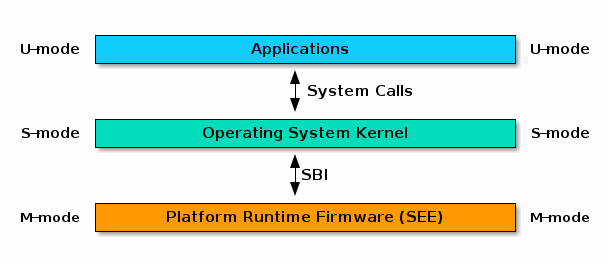
\includegraphics[width=0.7\linewidth]{assets/riscv-sbi-intro1.png}
\caption{不含H拓展的RISC-V系统}
\label{fig:riscv-sbi}
\end{figure}

如下为\texttt{arch/riscv/kernel/sbi.c}中的部分代码,使用\texttt{ecall}指令时,
将EID写在\texttt{a7} 寄存器,FID写在\texttt{a6}寄存器,参数写在 \texttt{a0}-\texttt{a5} 寄存器,
后面会根据EID和FID的不同调用不同的处理函数。
\begin{lstlisting}[language=C,numbers=left]
struct sbiret sbi_ecall(int ext, int fid, unsigned long arg0,
unsigned long arg1, unsigned long arg2,
unsigned long arg3, unsigned long arg4,
unsigned long arg5)
{
	struct sbiret ret;

	register uintptr_t a0 asm ("a0") = (uintptr_t)(arg0);
	register uintptr_t a1 asm ("a1") = (uintptr_t)(arg1);
	register uintptr_t a2 asm ("a2") = (uintptr_t)(arg2);
	register uintptr_t a3 asm ("a3") = (uintptr_t)(arg3);
	register uintptr_t a4 asm ("a4") = (uintptr_t)(arg4);
	register uintptr_t a5 asm ("a5") = (uintptr_t)(arg5);
	register uintptr_t a6 asm ("a6") = (uintptr_t)(fid);
	register uintptr_t a7 asm ("a7") = (uintptr_t)(ext);
	asm volatile ("ecall"
	: "+r" (a0), "+r" (a1)
	: "r" (a2), "r" (a3), "r" (a4), "r" (a5), "r" (a6), "r" (a7)
	: "memory");
	ret.error = a0;
	ret.value = a1;

	return ret;
}
\end{lstlisting}​

例如可以用如下程序实现一个打印一个字符到系统控制台上的\texttt{putchar}函数:
\begin{lstlisting}[language=C]
    void sbi_console_putchar(int ch)
    {
    	sbi_ecall(SBI_EXT_0_1_CONSOLE_PUTCHAR, 0, ch, 0, 0, 0, 0, 0);
    }
\end{lstlisting}

用SBI可以降低开发系统的难度,但是会引入\texttt{ecall}指令,而unikernel的高效正是
依靠避免\texttt{ecall}实现的,所以我们只会在前期使用SBI提供的服务,后期会用自己编写
的virtio驱动程序代替SBI。


\subsubsection{KVM对RISC-V架构的支持}
KVM (Kernel-based Virtual Machine,基于内核的虚拟机)  ,是一种内建于 Linux 中的
开源虚拟化技术。具体而言,KVM 可以将 Linux 转变为虚拟监控程序,从而使主机计算机能够运行
多个隔离的虚拟环境,即虚拟客户机或虚拟机(VM)。
\begin{figure}[!hbt]
	\centering
	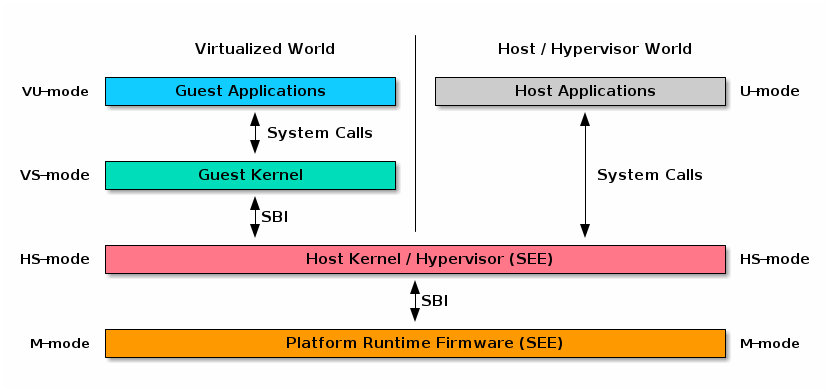
\includegraphics[width=0.9\linewidth]{assets/riscv-sbi-intro2.png}
	\caption{虚拟化下的特权等级}
	\label{fig:w4}
\end{figure}

如图\ref{fig:w4},为了支持虚拟化,RISC-V 规范定义了 RISC-V H-extension ,在原来的3级
特权架构的基础上对原有的 Supervisor 模式进行了扩展,引入了 Hypervisor-Extended Supervisor mode(HS)。
此时,在 Machine Mode 下运行最高优先级的、对全部资源具备操作能力的 Firmware ,虚拟机软件
Hypervisor 运行在 HS 模式,虚拟机 VM 运行在虚拟化的 Supervisor 模式,应用程序继续运行在
虚拟操作系统之上,运行在 Virtualized User mode。

为了实现 Supervisor 与 Hypervisor-extended supervisor 模式的切换,RSIC-V 将原来
Supervisor 模式下的 CSR 复制一份到Hypervisor,从而让每个硬件线程拥有两份 supervisor
寄存器,加快两个模式之间的切换过程。

由于 RISC-V 没有为不同虚拟化软件设计专门的特权模式,而是设计了统一的特权模式,这说明它对
1类(如Xvisor)、 2类(如KVM)虚拟化软件都有很好的支持。 RISC-V 可以通过 CSR 寄存器注入
中断,因此不需要为虚拟化而特殊设计中断控制器外设。此外,RISC-V 可直接借助特殊的寄存器位支持
嵌套虚拟化,而 Aarch64 要等到 v8.3 版本之后才支持这个功能。RISC-V 的时钟和核间中断可通过
SBI 软件辅助完成,而 Aarch64 需要特殊设计的计时器外设来支持虚拟化功能。\cite{bib:feasibility-d}

\subsection{QEMU}\sectionauthor{吴骏东}

QEMU是一款通用、开源的机器模拟器和虚拟化器。

当用作机器模拟器时,QEMU可以把一个机器(如ARM board)的系统或程序运行在不同的机器上(如你的PC)。
借助动态翻译,它达到了非常好的性能。

当用作虚拟化器时,QEMU通过直接在宿主机CPU上运行客户机代码,达到了接近原生的性能。QEMU支持两种模式
的虚拟化:在Xen hypervisor下执行,或者使用Linux内核模块KVM。当使用KVM时,QEMU可以虚拟化x86、
服务器和嵌入PowerPC、64位 POWER、S390、32位和64位ARM、RISC-V\cite{bib:qemu7}以及MIPS客户机。\cite{bib:feasibility-1}

\noindent QEMU具有如下优点:

\begin{description}
\item[完整系统的模拟] Run operating systems for any machine, on any supported architecture.
\item[用户态的模拟] Run programs for another Linux/BSD target, on any supported architecture.
\item[虚拟化] Run KVM and Xen virtual machines with near native performance.\cite{bib:feasibility-1}
\end{description}

\subsection{Unikraft架构分析}\sectionauthor{张子辰}\vspace*{-4ex}
\subsubsection{代码风格}\label{ssubsec:code-style}
Unikraft的代码组织方式充分体现了模块化设计,核心代码被放在了\texttt{arch/}、\texttt{include/}和
\texttt{plat/}三个目录下,而系统的几乎所有功能都由位于\texttt{lib/}目录下的micro-libraries提供。
一个micro-library被放在一个目录下:
\begin{itemize}
\item \texttt{include/}:micro-library的API;
\item \texttt{Config.uk}:menu-config配置;
\item \texttt{exportsyms.uk}:导出的符号;
\item \texttt{Makefile.uk}:自动构建系统的配置;
\item \texttt{*.c}:micro-library的实现。
\item \texttt{extra.ld}:(可选)链接器配置。
\end{itemize}

比如,\texttt{uksched}的目录结构:
{\linespread{1}
\begin{verbatim}
    uksched
    ├── Config.uk
    ├── exportsyms.uk
    ├── extra.ld
    ├── include
    │   └── uk
    │       ├── sched.h
    │       ├── thread_attr.h
    │       ├── thread.h
    │       ├── wait.h
    │       └── wait_types.h
    ├── Makefile.uk
    ├── sched.c
    ├── thread_attr.c
    └── thread.c
\end{verbatim}}

Unikraft用UNIX命名风格,函数名和结构体
以\texttt{uk\_\hspace{0cm}\textit{<micro-library\hspace{0cm}名\hspace{0cm}>}\hspace{0cm}\_}
开头,结构体名后\textit{通常}附加\texttt{\_t},
比如\texttt{uk\_malloc}、\texttt{uk\_alloc\_malloc\_func\_t}。
Unikraft使用面向对象设计,每个micro-library中通常有与库同名的结构体,如\texttt{uk\_sched},
库中的函数的第一个参数通常是执行这个结构体的指针,如
\texttt{\textbf{struct} uk\_sched *uk\_sched\_create(\textbf{struct} uk\_alloc *a, \textbf{size\_t} prv\_size)}。

\subsubsection{编译运行流程}
以编译\href{https://github.com/unikraft/app-helloworld}{hello world程序}为例,介绍编译并
运行基于Unikraft的unikernel的流程。

首先要修改\texttt{Makefile},把\texttt{UK\_ROOT}改为unikraft源代码的目录,比如
\texttt{UK\_ROOT ?= \linebreak\$(PWD)/../unikraft},当然也可以不修改\texttt{Makefile}而修改
命令行参数。

用\texttt{make menuconfig}配置,然后用\texttt{make}编译。
\begin{figure}[!hbt]
\centering
\vspace*{-3ex}
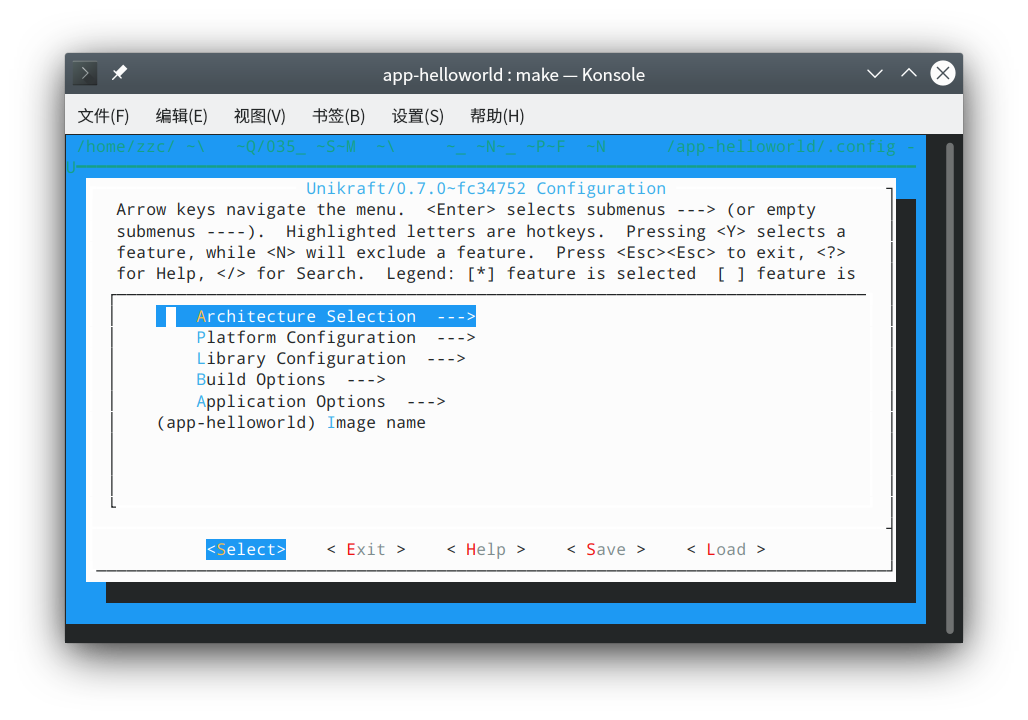
\includegraphics[width=0.9\linewidth]{assets/unikraft-menuconfig}
\vspace*{-3ex}
\caption{配置Unikraft}
\label{fig:unikraft-menuconfig}
\end{figure}
Hello world程序与Unikraft的各个被使用的micro-libraries先被分别编译成了\texttt{.o}文件,
再链接成一个unikernel镜像。一共生成了\texttt{libkvmplat}、\texttt{libkvmpci}、\texttt{libkvmvirtio}、
\texttt{apphelloworld}、\texttt{libnolibc}、\texttt{libukalloc}、\texttt{libukallocbbuddy}、
\texttt{libukargparse}、\texttt{libukboot}、\texttt{libukbus}、\texttt{libukdebug}、
\texttt{libuksglist}、\texttt{libuktime}、\texttt{libuktimeconv}和\texttt{libx86\_64arch}等中间文件。
最后的输出是18.0KiB大的\texttt{app-\linebreak helloworld\_kvm-x86\_64.gz}。

详细的编译日志位于我们的仓库的\href{https://github.com/OSH-2022/x-runikraft/tree/d22ccf0c1b248667148fd8953b71b6e0258de6a3/reference/Unikraft%20helloworld}{reference/Unikraft helloworld/}目录。

用\texttt{qemu-system-x86\_64 -kernel build/app-helloworld\_kvm-x86\_64 -nographic}\linebreak 运行hello world程序。

\begin{figure}[tbh!]
\centering
\vspace*{-3ex}
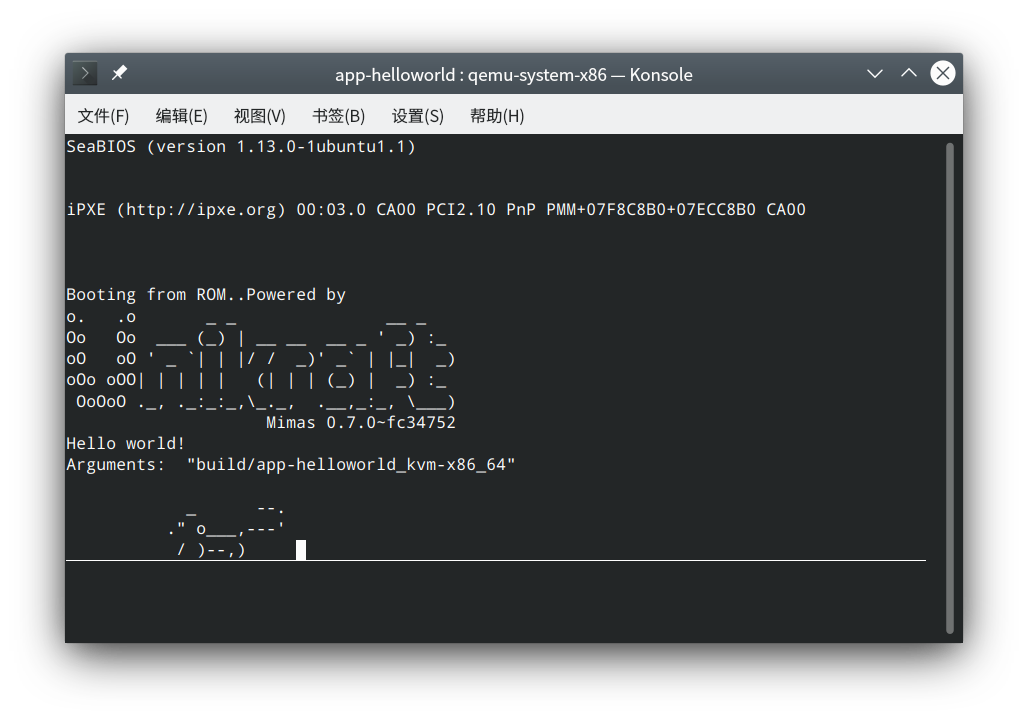
\includegraphics[width=0.9\linewidth]{assets/unikraft-run}
\vspace*{-3ex}
\caption{运行hello world}
\label{fig:unikraft-run}
\end{figure}


\subsubsection[开机流程]{开机流程(KVM+AMD64)}
\begin{enumerate}
\item bootloader(由虚拟机的固件实现)。
\item \texttt{\_libkvmplat\_start32}(位于\texttt{plat/kvm/x86/entry64.S}):
    \begin{enumerate}
    \item enable pae;
    \item enable long mode;
    \item load pml4 pointer;
    \item enable paging;
    \item \texttt{jmp \_libkvmplat\_start64}。
    \end{enumerate}
\item \texttt{\_libkvmplat\_start64}:
    \begin{enumerate}
    \item 一系列复杂的初始化;
    \item \texttt{call \_libkvmplat\_entry}。
    \end{enumerate}
\item \texttt{\_libkvmplat\_entry}(位于\texttt{plat/kvm/x86/setup.c}),
它接受\texttt{struct multiboot\_info*}参数:
    \begin{enumerate}
    \item \texttt{\_init\_cpufeatures};
    \item \texttt{\_libkvmplat\_init\_console};
    \item \texttt{traps\_init};
    \item \texttt{intctrl\_init};
    \item \texttt{\_mb\_get\_cmdline}:把multiboot\_info中的命令行参数复制到数据段
    的\texttt{char\linebreak cmdline[8192]};
    \item \texttt{\_mb\_init\_mem}:处理与内存分段有关的操作;
    \item \texttt{\_mb\_init\_initrd`};
    \item (\texttt{CONFIG\_HAVE\_SMP})\footnote{表示在开启某个配置时执行。} \texttt{acpi\_init};
    \item (\texttt{CONFIG\_HAVE\_SYSCALL}) \texttt{\_init\_syscall};
    \item (\texttt{CONFIG\_HAVE\_X86PKU}) \texttt{\_check\_ospke};
    调用\texttt{\_libkvmplat\_newstack}从引导栈切换走。
    \end{enumerate}
    可以看出,AMD64的开机流程很复杂,在ARMv8中,系统的起点是用汇编语言编写
    的\texttt{\_libkvmplat\_entry},它调用用C语言编写的\texttt{\_libkvmplat\_start},
    之后的流程与AMD64相同。
\item \texttt{\_libkvmplat\_entry2}:把cmdline传递给\texttt{ukplat\_entry\_argp}。
\item \texttt{ukplat\_entry\_argp}:把命令行参数拆成argc+argv的形式,然后调用\texttt{ukplat\_entry}。
\item \texttt{ukplat\_entry}:
    \begin{enumerate}
    \item 调用\texttt{ctorfn}注册的构造函数(\texttt{ctors.h}提供了注册构造函数的机制);
    \item (\texttt{CONFIG\_LIBUKLIBPARAM})进一步分析命令行参数;
    \item (\texttt{!CONFIG\_LIBUKBOOT\_NOALLOC}) 依次尝试在每一块内存区域上初始化
    分配器\linebreak(\texttt{uk\_<name>\_init}),
    成功创建分配器后,将剩余的内存区域加入分配器\linebreak(\texttt{uk\_alloc\_addmem});
    \item (\texttt{CONFIG\_LIBUKALLOC}) 初始化中断(\texttt{ukplat\_irq\_init});
    \item (\texttt{CONFIG\_LIBUKSCHED}) 初始化调度器\texttt{uk\_sched\_default\_init};
    \item (\texttt{CONFIG\_LIBUKSCHED}?)
        \begin{itemize}
        \item (true)  创建主线程(执行\texttt{main\_thread\_func})→启动调度器(\texttt{uk\_sched\_start}),
        \item (false) 启动中断(\texttt{ukplat\_lcpu\_enable\_irq})→直接调用\texttt{main\_thread\_func}。
        \end{itemize}
    \end{enumerate}
\item \texttt{main\_thread\_func}:
    \begin{enumerate}
    \item 调用init table上注册的函数(由\texttt{init.h}提供,与\texttt{ctorfn}类似);
    \item (\texttt{CONFIG\_LIBUKSP})\texttt{uk\_stack\_chk\_guard\_setup};
    \item 调用用户程序的构造函数 \texttt{\_\_preinit\_array}和\texttt{\_\_init\_array};
    \item 调用用户程序的\texttt{main}。
    \end{enumerate}
\item \texttt{main}。
\item 关机/崩溃。
\end{enumerate}

\subsubsection{分配器}
分配器的API位于\texttt{ukalloc},可选的实现有\texttt{ukallocbbuddy}、\texttt{ukallocpool}、
\texttt{ukallocregion}。\texttt{ukalloc}用函数指针实现了类似C++的虚函数的运行时绑定,其他的
Unikraft 接口micro-libraries也采用了类似的技术。\texttt{\textbf{struct} uk\_alloc}保存
\texttt{malloc}、\texttt{free}等指向实现的函数指针,\texttt{uk\_malloc}等接口函数
接受\texttt{uk\_alloc}型指针\texttt{a},将参数转发给\texttt{a}的函数指针。比如,\texttt{malloc}的
实现:
\begin{lstlisting}[language=C]
static inline void *uk_do_malloc(struct uk_alloc *a, __sz size)
{
	UK_ASSERT(a);
	return a->malloc(a, size);
}

static inline void *uk_malloc(struct uk_alloc *a, __sz size)
{
	if (unlikely(!a)) {
		errno = ENOMEM;
		return __NULL;
	}
	return uk_do_malloc(a, size);
}
\end{lstlisting}

具体的实现负责初始化\texttt{uk\_alloc}变量,比如\texttt{ukbbuddy}实现了伙伴分配器,它提供的
\texttt{struct uk\_alloc *uk\_allocbbuddy\_init(void *base, size\_t len)}函数会把
自己的实现绑定到\texttt{uk\_alloc}中的函数指针。

\subsubsection{调度器}
调度器API位于\texttt{uksched},它主要包括\texttt{sched}和\texttt{thread}两个子模块。

\texttt{thread}既是接口又是实现,它提供针对单个线程的操作,
其中的\texttt{\textbf{struct} uk\_thread}保存线程控制块,
\texttt{uk\_thread\_set\_timeslice}函数设置线程时间片,\texttt{uk\_thread\_wake}
函数唤醒线程,根据线程的时间片设置定时器,然后把控制权转交给这个线程,这些操作需要调用\texttt{ukplat}
的API。

\texttt{sched}是只是接口,它
负责管理所有线程,它调用\texttt{thread}的API操作单个线程。
\texttt{ukschedcoop}是\texttt{uksched}的实现之一,它实现了最基本非抢占式的时间片轮转线程调度器。
它使用双链尾队列(tail queue)维护所有线程(\texttt{thread\_list})和
睡眠状态(就绪或等待)的线程(\texttt{sleeping\_threads})。
每一轮调度,\texttt{ukschedcoop}从睡眠线程队列
中找出一个处在就绪态的线程,并唤醒(\texttt{uk\_thread\_wake})这个线程。
如果没有任何能执行的线程,就挂起CPU(\texttt{ukplat\_lcpu\_halt\_to}),
直到某个线程能执行。\texttt{ukschedcoop}并不需要为每一个事件维护等待队列,
因为即使线程等待的事件发生了,由于当前线程的执行不能被抢占,等待的线程也不能被立即唤醒。

Unikraft的论文中提到了它拥有抢占式调度器\texttt{ukpreempt},但是我们并没有在它的源代码中找到相应的实现。

\section{技术依据}\sectionauthor{张子辰}\vspace*{-4ex}
\subsection{rustc交叉编译}
先安装交叉编译riscv64gc的编译器组件,
然后在编译时附加\texttt{--target riscv64gc-\linebreak unknown-none-elf}选项即可实现x86-64--riscv64交叉编译。

还需要安装\texttt{rust-objcopy}以生成QEMU能加载的原始二进制文件。

\noindent 命令(假定已安装通过rustup安装Rust构建工具链):
\begin{lstlisting}
rustup target add riscv64gc-unknown-none-elf
cargo install cargo-binutils
\end{lstlisting}

\subsection{启动操作系统}
添加编译选项\texttt{-Clink-arg=-Tlinker.ld}以便链接器能读取自定义的链接脚本:
\begin{multicols}{2}
\begin{lstlisting}[numbers=left]
OUTPUT_ARCH(riscv)
ENTRY(__runikraft_start)
BASE_ADDRESS = 0x80200000;

SECTIONS
{
    . = BASE_ADDRESS;
    skernel = .;

    stext = .;
    .text : {
        *(.text.entry)
        *(.text .text.*)
    }

    . = ALIGN(4K);
    etext = .;
    srodata = .;
    .rodata : {
        *(.rodata .rodata.*)
        *(.srodata .srodata.*)
    }

    . = ALIGN(4K);
    erodata = .;
    sdata = .;
    .data : {
        *(.data .data.*)
        *(.sdata .sdata.*)
    }

    . = ALIGN(4K);
    edata = .;
    .bss : {
        *(.bss.stack)
        sbss = .;
        *(.bss .bss.*)
        *(.sbss .sbss.*)
    }

    . = ALIGN(4K);
    ebss = .;
    ekernel = .;

    /DISCARD/ : {
        *(.eh_frame)
    }
}
\end{lstlisting}
\end{multicols}

初始化函数需要用汇编语言编写:
\begin{lstlisting}[numbers=left]
.extern sbss
.extern ebss

.section .text.entry
.globl __runikraft_start

__runikraft_start:
    #清空bss段
    la t0,sbss
    la t1,ebss
    clean_bss:
        bge t0,t1,clean_bss_end
        sd x0,(t0)
        addi t0,t0,8
        j clean_bss
    clean_bss_end:
    addi t0,zero,0
    addi t1,zero,0
    #加载栈指针
    la sp,stack_top
    call __runikraft_entry_point

.section .bss.stack
    .space 65536
stack_top:
\end{lstlisting}
它加载栈指针,然后将控制权转交给用Rust写的更高层的初始化函数。目前后者还只有雏形,它只初始化\texttt{rk::plat}模块
的定时器子模块,然后调用用户程序的入口\texttt{main}。
\begin{lstlisting}[language=Rust,numbers=left]
/// 系统的入口,由引导程序调用
///
#[no_mangle]
pub fn __runikraft_entry_point()->!{
    time::init();
    unsafe{main();}
    halt();
}
\end{lstlisting}

\texttt{\_\_runikraft\_entry\_point}和\texttt{\_\_runikraft\_start}都是Runikraft核心组件的
\texttt{plat::\linebreak bootstrap}的一部分,目前的核心组件还实现了\texttt{plat::console}和
\texttt{plat::time}两个\texttt{plat}模块的子模块,以及\texttt{bitcount}模块(这个模块完全是
对Unikraft的\texttt{bitcount.c}的翻译)。目前已经实现了\texttt{rkalloc} API(对应Unikraft的
\texttt{ukalloc},这个API有一个演示用的“空实现”\texttt{rkalloc\_empty}。

目前的\texttt{main}函数能简单演示\texttt{plat::console}、\texttt{plat::time}和\texttt{rkalloc}:
\begin{lstlisting}[language=Rust,numbers=left]
#![no_std]
#![no_main]

use runikraft as rk;

use rkalloc::Alloc;
use rkalloc_empty::RKallocEmpty;
use rk::plat::time;

static mut HEAP_SPACE: [u8;1000] = [0;1000];

#[no_mangle]
fn main() {
    let mut alloc;
    unsafe {
        alloc = RKallocEmpty::new(HEAP_SPACE.as_mut_ptr(),1000);
    }
    rk::println!("Hello, world!");
    let p1 = unsafe{alloc.malloc(10)};
    rk::println!("p1={:?}",p1);
    let p2 = unsafe{alloc.malloc(5)};
    rk::println!("p2={:?}",p2);
    rk::println!("sleep for 10s");
    let start = time::get_ticks();
    loop {
        if (time::get_ticks() - start).as_secs()>=10 {break;}
    }
    let end = time::get_ticks();
    rk::println!("slept for {:?}",end - start);
}
\end{lstlisting}

\subsection{编译}
依次运行
\begin{lstlisting}
cargo build --release
rust-objcopy --strip-all build/riscv64gc-unknown-none-elf/release/dev-test -O binary build/riscv64gc-unknown-none-elf/release/dev-test.bin
\end{lstlisting}
即可完成编译。

\subsection{运行和调试}
这一步需要QEMU \texttt{riscv64}、\texttt{riscv64-unknown-elf} GDB和OpenSBI的
\texttt{fw\_jump.bin}。QEMU可以用\texttt{sudo apt install qemu-system-misc}安装,
当然也可以用\texttt{sudo apt install qemu-system}完整地安装QEMU。符合要求的GDB并没有
被收录在Ubuntu的软件源中,幸好SiFive提供了一套预编译的调试工具链,其可在\
\href{https://github.com/sifive/freedom-tools/releases}{sifive/freedom-tools}\
下载。下载并解压后,可以将\texttt{riscv64-unknown-elf-toolchain-10.2.0-2020.12.8-x86\_64-linux-ubuntu14/bin}添加到\texttt{PATH}。
QEMU的文档声称已经附带了\texttt{OpenSBI}\cite{bib:qemu-virt},
但是Ubuntu 20.04的APT源中的QEMU并没有附带,所以仍然需要到
\ \href{https://github.com/riscv-software-src/opensbi/releases/tag/v1.0}{OpenSBI Version 1.0}\
手动下载。我们需要的是\linebreak\texttt{opensbi-1.0-rv-bin/share/opensbi/lp64/generic/firmware/fw\_jump.bin}。
为了方便后续使用,可以在\texttt{\tildechar/.bashrc}中加上\texttt{export RISCV\_BIOS=\textit{<PATH\_TO\_fw\_jump.bin>}}。

一切安装完毕后,可以用
\begin{lstlisting}
qemu-system-riscv64 -machine virt -nographic -bios $RISCV_BIOS -device loader,file=build/riscv64gc-unknown-none-elf/release/dev-test.bin,addr=0x80200000 -s -S
\end{lstlisting}
启动系统。用
\begin{lstlisting}
riscv64-unknown-elf-gdb -ex 'file build/riscv64gc-unknown-none-elf/release/dev-test' -ex 'set arch riscv:rv64' -ex 'target remote localhost:1234'
\end{lstlisting}
进行交互式调试。

\begin{figure}[tbh!]
\centering
\vspace*{-3ex}
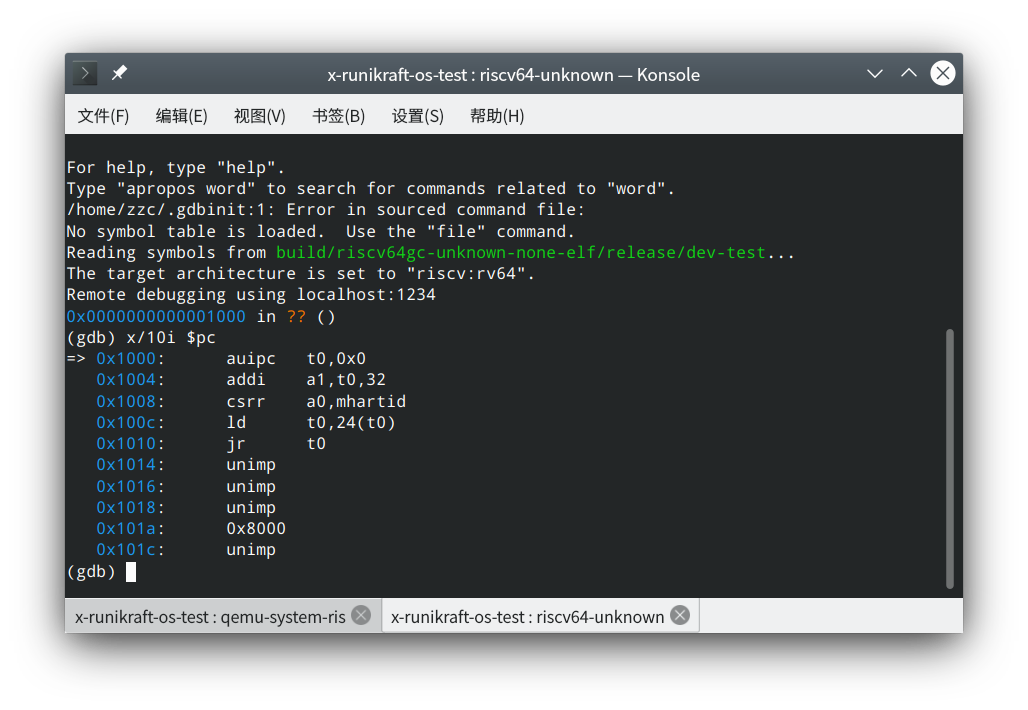
\includegraphics[width=0.9\linewidth]{assets/debug.png}
\vspace*{-3ex}
\caption{调试}
\label{fig:debug}
\end{figure}

\begin{figure}[tbh!]
\centering
\vspace*{-3ex}
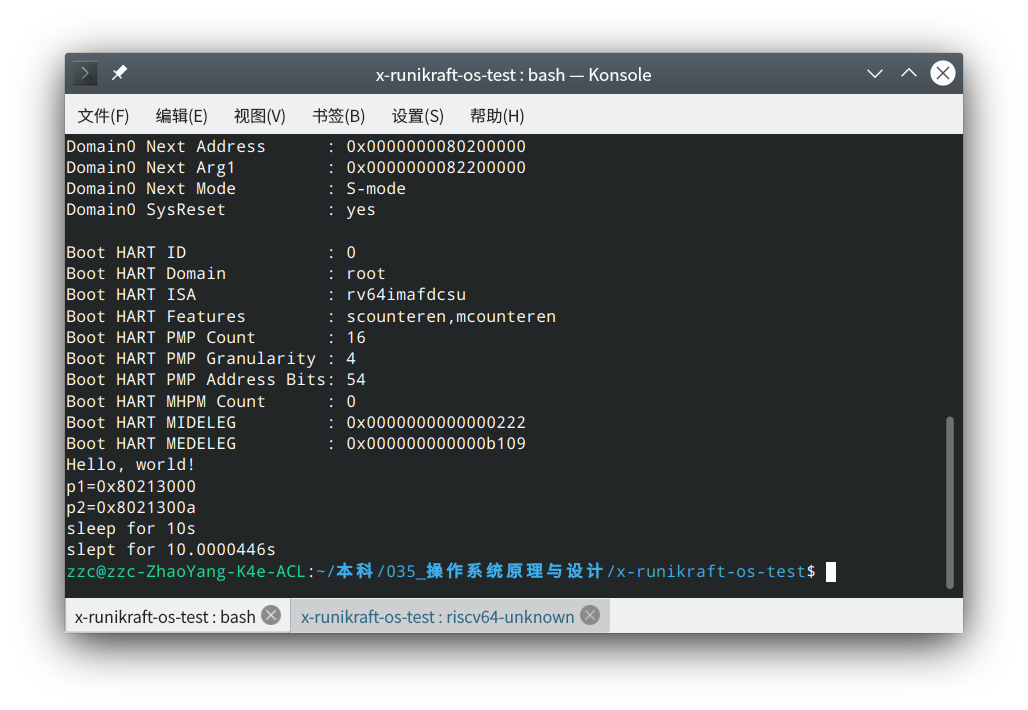
\includegraphics[width=0.9\linewidth]{assets/run.png}
\vspace*{-3ex}
\caption{运行结果}
\label{fig:run}
\end{figure}

\begin{comment}

\subsection{Unikernel}
Unikernel是专一用途的、单地址空间的轻量操作系统。Unikernels在虚拟机
上运行时,能够提供比传统的容器更短的启动时间、更高的运行效率和更强的
隔离性,因rn此unikeels通常被用在云计算领域。\cite{bib:unikernel}


\noindent 现有的unikernels普遍存在以下问题:\cite{bib:unikraft}
\begin{itemize}
\item 编译它们并让它们达到高效率需要大量专业的工作,而且这些工作通常
需要对每个目标应用程序重做。
\item 它们通常不是POSIX兼容的,需要移植程序和语言环境。
\end{itemize}

\ref{subsec:famous-unikernel-projects}\ 小节将简要介绍我们小组详细调研的ClickOS、MirageOS、IncludeOS、Rusty-Hermit、Rumprun
和Unikraft等六个目前仍然在维护的unikernel项目。
\end{comment}

\section{前瞻性/重要性分析}

\subsection{使用先进的工具构建}\sectionauthor{郭耸霄 and 张子辰}

Rust和RISC-V都是新兴事物,它们都是在吸取旧事物的教训的基础上诞生的,
而且,实践表明,两者都正在经历蓬勃的发展,并正在分别逐步取代旧事物。
因此,用Rust在RISC-V上开发unikernel顺应了历史的趋势。

Rust 是由 Mozilla 研究室
主导开发的一门现代系统编程语言,自 2015 年 5 月发布 1.0 之后,一直以每 6 周
一个小版本的开发进度稳定向前推进。语言设计上跟 C++ 一样强调零开销抽象和 RAII。
拥有极小的运行时和高效的 C 绑定,使其运行效率与 C/C++ 一个级别,非常适合对性能
要求较高的系统编程领域。利用强大的类型系统和独特的生命周期管理实现了编译期内存管理,
保证内存安全和线程安全的同时使编译后的程序运行速度极快,Rust 还提供函数式编程语言
的模式匹配和类型推导,让程序写起来更简洁优雅。\cite{bib:2-why-rust}
总地来说,Rust是一门赋予每个人 构建可靠且高效软件能力的语言。\cite{bib:1-rust-lang}
Rust具有高性能、可靠性、生产力三方面的优势。

RISC-V是于2010年诞生自加州大学伯克利分校的精简指令集架构,
它的目标是成为一个通用的指令集架构,它能适应包括从最袖珍的嵌入式控制器,
到最快的高性能计算机等各种规模的处理器;它能兼容各种流行的软件栈和编程语言;
它能适应所有实现技术,包括现场可编程门阵列(FPGA)
 、专用集成电路(ASIC) 、全定制芯片,甚至未来的设备技术;它对所有微体系结构样式都有效,
例如微编码或硬连线控制、顺序或乱序执行流水线、单发射或超标量等;它支持广泛的专业化,
成为定制加速器的基础;它是稳定的,基础的指令集架构不应该改变。\cite{bib:risc-v-manual}
与以往的ISA不同,RISC-V是\textit{模块化}的。它的核心是一个名为RV32I的基础ISA,
运行一个完整的软件栈。RV32I是固定的,永远不会改变。这为编译器编写者,操作系统开发人员和汇
编语言程序员提供了稳定的目标。模块化来源于可选的标准扩展,根据应用程序的需要,
硬件可以包含或不包含这些扩展。这种模块化特性使得RISC-V具有了袖珍化、低能耗的特
点,而这对于嵌入式应用可能至关重要。RISC-V在设计时考虑了成本、简洁性、性能、
架构和具体实现的分离、提升空间、
程序大小和易于编程/编译/链接七个方面的因素。

目前的unikernel中,使用/支持两者中的一个的都很少,而根本没有将两者结合者。Runi\-kraft的
亮点之一就是将两者结合。

\subsection{模块化设计}\sectionauthor{张子辰}
目前的大多数unikernel强调“uni-”,它们的设计者认为这样有利于提高效率,
所以系统被设计成了一个整体,这个整体向用户提供能够调用函数。具体的表现就是
系统的源代码堆在一起,ClickOS、IncludeOS、MirageOS、RustyHermit都有这样
的问题。系统缺乏明确的功能组件,所以系统必须作为一个整体维护。

在Runikraft中,只有极少数平台层的代码被放到了系统的核心组件中,而调度器、
分配器等组件一律是micro-libraries。这些micro-libraries遵循一套明确
定义的APIs,同一个系统模块可以有多种实现,用户可以轻松为自己的需求选择合适的系统组件的实现。
从Unikraft给出的基准测试数据看,这种模块划分不会降低系统的效率。

\subsection{创新点}
与先前用Rust改写FreeRTOS的小组类似,我们的项目偏重工程,没有理论上的创新点。
由于我们了解的所有用Rust写的操作系统都或多或少的使用了unstable的特性,我们用stable特性
编写unikernel也不失为一种技术上的创新。

\section{概要设计}\sectionauthor{张子辰}
\begin{figure}[!hbt]
\centering
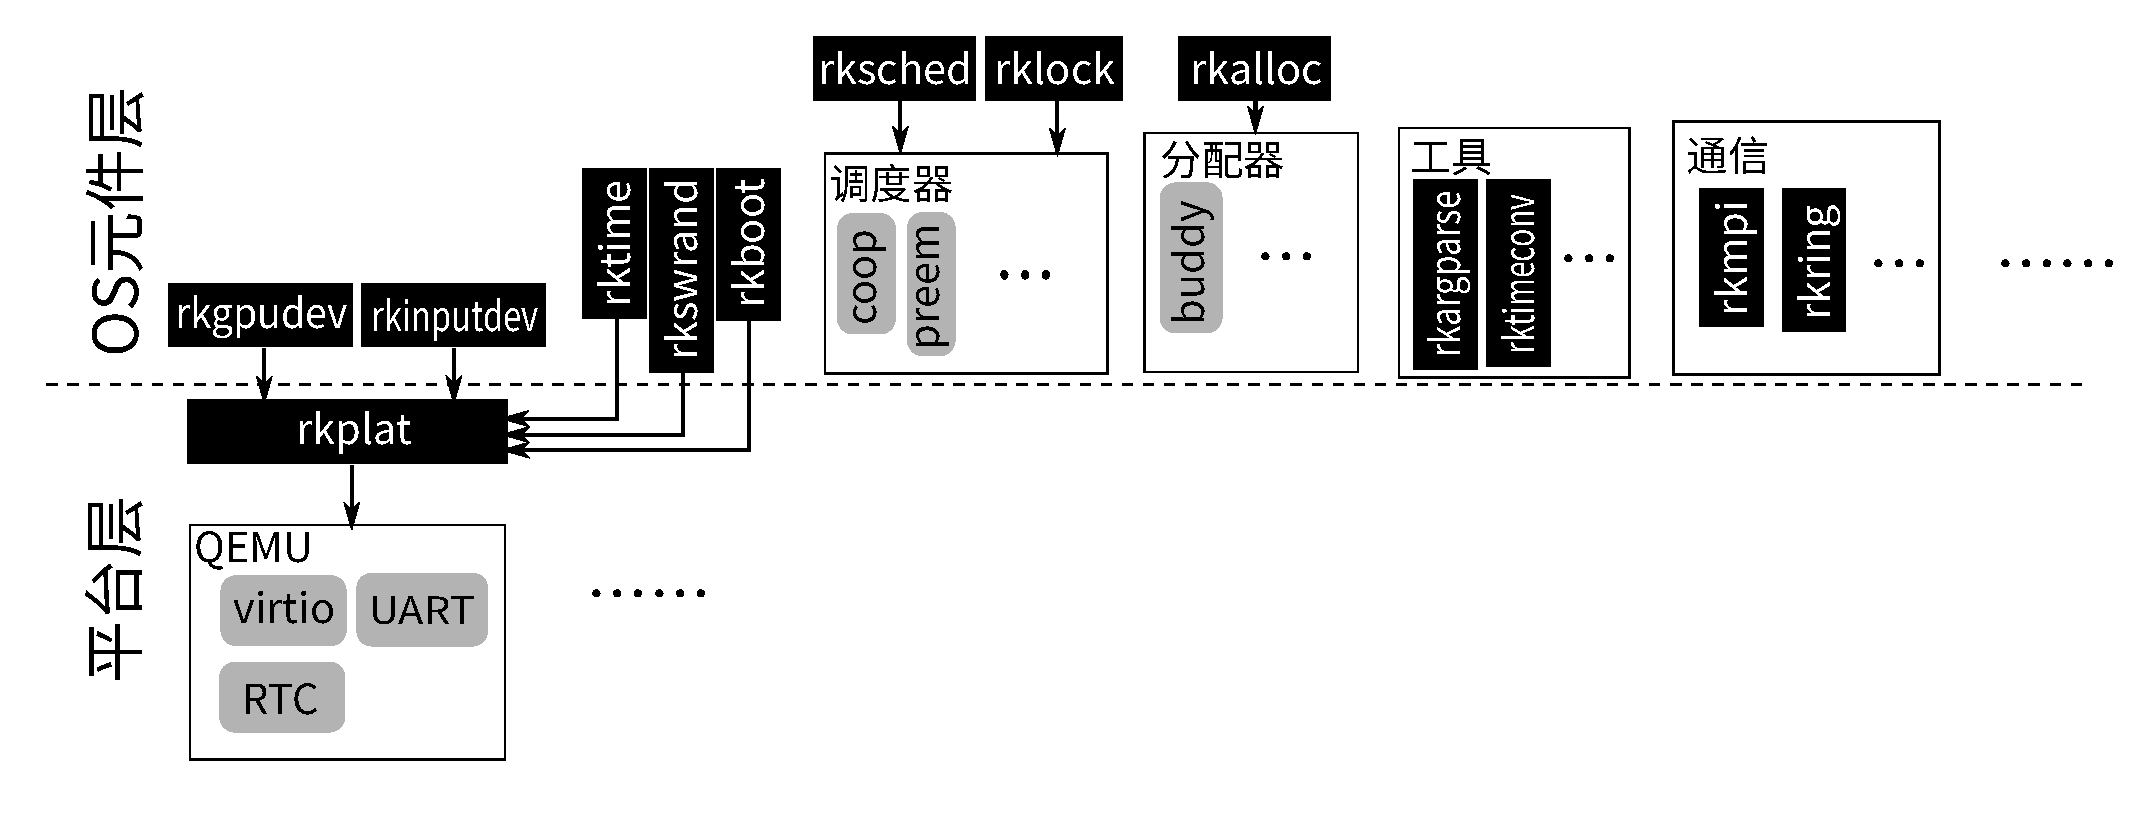
\includegraphics[width=\linewidth]{assets/Runikraft-architecture-impl.pdf}
\caption{Runikraft的架构}\label{fig:runikraft-arch-impl}
\end{figure}
平台层将不同的平台封装成通用的\texttt{rkplat} API,它提供与平台/架构密切相关的功能,
比如外设驱动、外中断处理、内存分页、定时器、原子操作、内存屏障,我们只支持RISC-V+QEMU virt
一种平台。对于RISC-V架构,OSes运行在supervisor特权模式,它需要运行在machine特权模式的
OpenSBI\cite{bib:feasibility-5}\cite{bib:feasibility-6}的协助才能关机、设置定时器和
触发核间中断。

\texttt{rkgpudev}、\texttt{rkinputdev}、\texttt{rktime}、\texttt{rkswrand}、\texttt{rkboot}
五个APIs的功能与平台密切相关,
但是为了降低开发和维护难度,它们并没有直接实现,而是在\texttt{rkplat}提供的初级抽象的基础上实现。
\texttt{rkgpudev}和\texttt{rbintputdev}分别提供显示设备和输入设备的支持。
\texttt{rktime}提供获取系统时间的API,\texttt{rkswrand}提供密码学安全的随机数,
\texttt{rkboot}负责完成OS元件的初始化并将控制权交给用户的代码。

\texttt{rksched}和\texttt{rklock}是两个与调度器有关的APIs,前者负责创建、调度、撤销线程,后者负责线程间
的同步和互斥。Runikraft支持多种调取器,比如,图\ \ref{fig:runikraft-arch-impl}\ 中的
coop是协作式的FCFS调度器、
preem是抢占式的RR调度器。当然,为了系统镜像的轻量性,用户可以不使用任何调取器。

Runikraft选择性地提供线程通信模块,如基于信箱的线程通信(\texttt{rkmpi}),
无锁的环形缓冲队列(\texttt{rkring})。
Runikraft不区分线程和进程,它的线程同时具有传统的OSes的线程和进程的特性:
线程之间没有隔离措施,但是线程之间又可以使用进程通信的方法更安全地同步。

\texttt{rkalloc}是分配器API,它的后端可以是\texttt{buddy}、\texttt{tinyalloc}、\texttt{tlsf}、
\texttt{mimalloc}等分配器。
目前,我们只实现了其中的\texttt{buddy},即伙伴分配器。

Runikraft还提供了一些工具模块,比如时间格式转换工具\texttt{rktimeconv}、
命令行参数分析工具\texttt{rkargparse}。我们曾经计划实现调试工具\texttt{rkdebug},但我们发现,
Rust的核心库提供的\texttt{assert}和\texttt{debug\_assert}宏已经足够取代Unikraft的\texttt{ukdebug}了,
所以最终没有实现。

\begin{table}[!hbt]
\caption{Unikraft与Runikraft的组件的对应}
\centering
\begin{tabular}{lll}
\hline
Unikraft&Runikraft&功能\\\hline
\texttt{ukalloc}&\texttt{rkalloc}&分配器API\\
\texttt{ukallocbuddy}&\texttt{rkallocbuddy}&分配器实现——伙伴分配器\\
\texttt{ukargparse}&\texttt{rkargparse}&kernel arguments parsing\\
\texttt{ukboot}&\texttt{rkboot}&初始化系统\\
(无)&\texttt{rkgpudev}&显示设备\\
\texttt{uklock}&\texttt{rklock}&互斥锁、信号量\\
\texttt{ukmpi}&\texttt{rkmpi}&基于信箱的通信\\
\texttt{ukplat}&\texttt{rkplat}&平台相关代码\\
\texttt{ukring}&\texttt{rkring}&无锁环形缓冲区\\
\texttt{uksched}&\texttt{rksched}&调度器API\\
\texttt{ukschedcoop}&\texttt{rkschedcoop}&调度器实现——FCFS\\
(无)&\texttt{rkschedpreem}&调度器实现——RR\\
\texttt{ukswrand}&\texttt{rkswrand}&密码学安全的随机数生成器\\
\texttt{uktimeconv}&\texttt{rktimeconv}&时间格式转换\\
\hline
\end{tabular}
\end{table}

\begin{figure}[!htb]
\centering
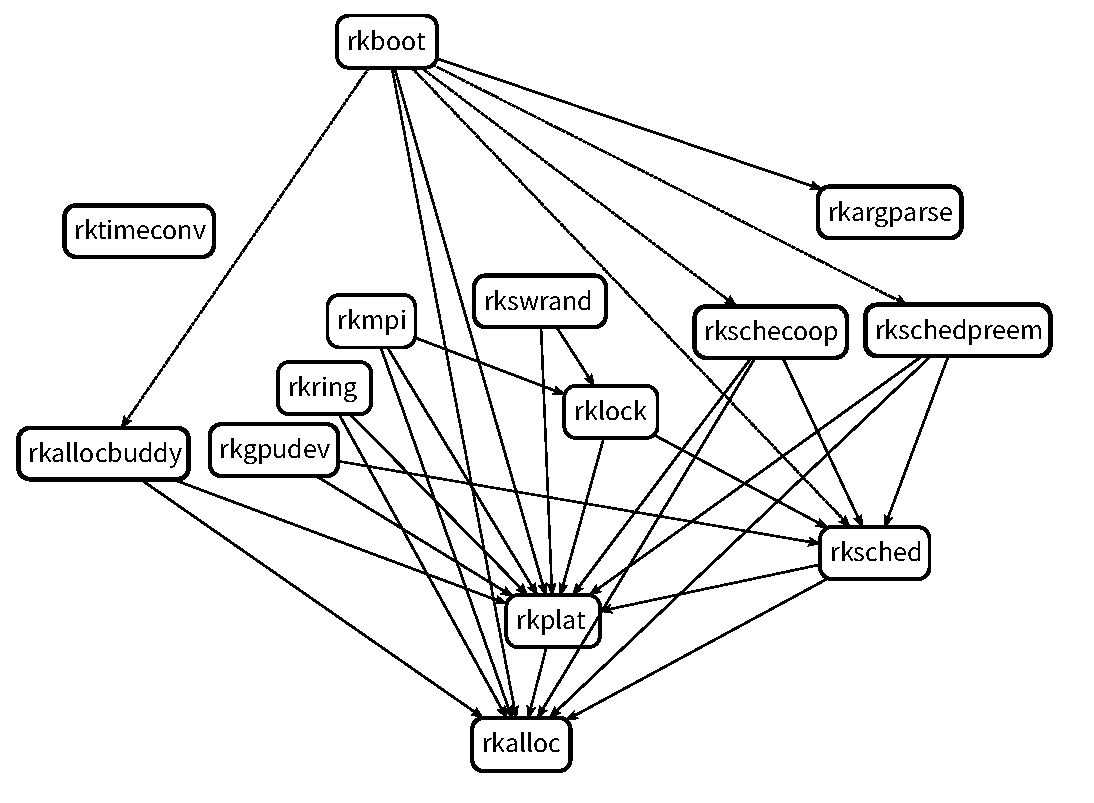
\includegraphics[width=\linewidth]{assets/crates-dependency.pdf}
\caption{Runikraft的crates的依赖关系}
\end{figure}

\section{功能组件}\sectionauthor{张子辰}
本节介绍Runikraft的重要crates的设计思想,不展示具体的APIs,也不介绍容易实现的次要组件。
\subsection[\texttt{rkplat}]{\texttt{rkplat}:平台相关代码}
\texttt{rkplat}主要包含\texttt{console}、\texttt{irq}、
\texttt{lcpu}、\texttt{thread}和\texttt{time}等模块。

\texttt{console}提供最基本的控制台输入输出,包括Unikraft风格的\texttt{cink}、\texttt{coutk}和Rust
风格的\texttt{print}、\texttt{println}。

\texttt{irq}是中断子系统。在异常/中断发生后,\texttt{\_\_rkplat\_int\_except\_entry}将
判断发生的是异常还是中断。对于异常,所有寄存器都会被保存到一段相对不容易被破坏的内存区域,然后
\texttt{\_\_rkplat\_exception\_handle}会输出异常信息。对于中断,只有\texttt{t*}和\texttt{a*}
寄存器会被保存到当前在栈上,然后控制权会被交给中断子系统的\texttt{\_\_rkplat\_irq\_handle}函数,
后者会调用有平台无关代码事先注册的中断响应函数。

\texttt{lcpu} 处理逻辑处理器,包括但不限于关闭/开启中断,获取当前的逻辑处理器的编号,唤醒另一个
逻辑处理器,读取栈指针。

\texttt{thread}提供切换和启动线程的原语\texttt{start(A)}和\texttt{switch(A,B)}。\texttt{start}将执行流
转到一个从未运行过的线程A。\texttt{switch}将执行流从线程A切换到另外一个调用了\texttt{switch}
或从未执行过的线程B。1. 如果线程B从未执行过,那么执行流将转到B的入口;2. 如果线程B先前调用
了\texttt{switch},那么执行流将转到B线程的\texttt{switch}函数后的指令,这意味着,
B线程会观察到\texttt{switch}函数返回。无论哪种情况,线程A会被挂起到某一个线程调用\texttt{switch}切换到A。
\texttt{switch}函数实现了“自主”的线程切换,相比传统的OSes中的需要supervisor协助的线程切换,这种模式减少了
一次上下文切换,因此更快速地完成线程的切换。%在介绍\texttt{rksched}的设计时,将详细介绍Runikraft的线程模型。

\texttt{rktime}负责查询时间和设置定时器。

总体来说,\texttt{rkplat}提取了多种ISAs的共性,隐藏了不同的ISAs之间的差异,使 Runikraft的
其他crates的代码能不依赖特定的ISA。
\subsection[\texttt{rkalloc}]{\texttt{rkalloc}:分配器}
分配器的API位于\texttt{rkalloc} crate,实现之一是\texttt{rkallocbuddy}。

\texttt{rkalloc} API兼顾了Rust风格的分配器和C风格的分配器。首先,\texttt{Alloc} trait
的接口与\texttt{alloc::alloc::GlobalAlloc}很接近,在解分配时,必须提供分配时使用的\texttt{size}
和\texttt{align},这能降低实现分配器的难度。其次,\texttt{AllocExt} trait提供与C的\texttt{free}
兼容的解分配函数\texttt{dealloc\_ext(ptr: *mut u8)},在解分配时,只需要提供一个指针。

\texttt{rkallocbuddy}是伙伴分配器,它实现了\texttt{AllocExt} trait。尽管我们可以轻松地
在Internet上找到多种伙伴分配器的C实现\cite{bib:buddy-C-1}\cite{bib:buddy-C-2}\cite{bib:buddy-C-3}和Rust实现\cite{bib:buddy-Rust-1}\cite{bib:buddy-Rust-2}\cite{bib:buddy-Rust-3},
但是它们都不完全符合Runikraft的要求。
这是因为Rust的实现以实现\texttt{GlobalAlloc} trait为目标,不支持\texttt{AllocExt};
一些C的实现虽然非常精彩,但是需要改写成Rust才能使用。所以我们选择自行实现伙伴分配器。

首先考虑大小为$2^n$的被管理的内存区域。

最小的块的长度是$2^4$ bytes,能容纳2个指针;最大的块的大小为$2^{48}$ bytes,是AMD64支持的最大内存容量。
用双向链表维护空闲块,链表的结点\texttt{Node}储存在它对应的内存区域的开头。
用树状bitset维护所有的内存区块的分配情况(元数据):
\begin{itemize}
\item \texttt{[0]}是根结点;
\item \texttt{[i*2+1]}是\texttt{[i]}的左孩子,它对应的内存区域是\texttt{i}二分后的前半段;
\item \texttt{[i*2+2]}是\texttt{[i]}的右孩子,它对应的内存区域是\texttt{i}二分后的后半段;
\item 顺序(order)等于\texttt{k}的结点在这个bitset的索引范围是\texttt{[$2^{n-k}-1$:$2^{n-k+1}-2$]};
\item 顺序等于\texttt{k}的结点共有$2^{n-k}$个,每个的大小等于$2^k$;
\item 整个bitset的大小等于$2^{n+1}\div16\div8=2^{n-6}$ bytes
\item \texttt{bitset[i]} = 0 表示结点i:
    \begin{itemize}
        \item i 没有被分配,
        \item i 的父结点已经被分配;
    \end{itemize}
\item \texttt{bitset[i]} = 1 表示结点i:
    \begin{itemize}
        \item i 被分配,
        \item i 被二分成了两个子结点。
    \end{itemize}
\end{itemize}
初始时,元数据的所有位都是0,如果一块内存i被分配,则i的孩子一定全是0,i和i的祖先一定全是1。

元数据被储存在被管理的内存区块的末尾,它们需要占用$2^{n-10}$个最小的块。

当内存区域的大小size不是2的幂时,记$n=\lceil\log_2(\mathrm{size})\rceil$,
则可以将内存区域视为大小为$2^n$但末尾的一些
结点已经被分配的内存区域。

\subsection[\texttt{rksched}]{\texttt{rksched}:调度器}
调度器的API位于\texttt{rksched} crate,
实现有\texttt{rkschedcoop}、\texttt{rkschedpreem}。

在Runikraft中,调度器由\texttt{Thread}、\texttt{Sched}和\texttt{WaitQ}等三个密切
配合的结构体实现。\texttt{Thread}保存线程的控制块,\texttt{Sched}按照一定的顺序将CPU时间
分配给线程,\texttt{WaitQ}维护事件的等待队列。

\texttt{Thread}的重要成员有栈顶指针、thread local storage指针、状态(detached、ended、runnable)、
属性(优先级、时间片长度、截止时间等)、占用的资源上限(CPU时间、内存空间等)和指向控制线程的调度器的
裸指针。直接使用\texttt{Thread}既不方便也不安全:首先,需要分配线程栈空间(stack)和线程本地存储空间(tls)。
接着需对tls的低地址调用\texttt{init}(\texttt{unsafe\{*(tls as *mut Thread).init(...)\}}),初始化控制块,
\texttt{init}的tls参数应等于\texttt{tls+size\_of::<Thread>}。
之后用\texttt{add\_thread}把线程加入调度器。调度器将周期性地执行线程,直到线程执行完毕或被killed,这时
必须调用\texttt{exit}。\texttt{exit}函数会invoke调度器,切换到另一个没有退出的线程。然后,调度器会
调用\texttt{finish},唤醒等待这个线程结束的线程。如果线程是detached,调度器将释放线程的栈空间和thread local
storage,对于joinable线程,创建线程的线程负责释放空间。考虑到\texttt{Thread}的API非常不易用,
Runikraft提供了\texttt{create\_thread}和\texttt{destroy\_thread}两个能够安全地创建和销毁线程的函数。

\texttt{Thread}对象自身其实是\texttt{Tailq}的结点,这样可以通过修改指针的方式把线程加入或移出就绪队列。
不过,\texttt{WaitQ}是Thread的\textit{地址}构成的\texttt{Stailq},而不是\texttt{Thread}自身
构成的\texttt{Tailq},
这样做是为了使一个线程能够同时等待多个事件,并且在其中任意一个事件发生时被唤醒。每将线程加入等待队列,
都需要创建\texttt{StailqNode<NonNull<Thread>>}对象。为了不使用分配器,这个对象被创建在了栈上,
这意味着,需要将执行栈对象的指针传递出去。这是安全的,因为线程被加入等待队列后,会被立即挂起,栈中的对象
不会被dropped,当且仅当线程被唤醒,\texttt{StailqNode<...>}对象被移出等待队列后,创建在堆
上的\texttt{StailqNode<...>}对象才会被dropped。

\texttt{Sched}是trait,它的重要公开接口有\texttt{start}、\texttt{yield}、\texttt{add\_thread}、
\texttt{remove\_thread}、\linebreak\texttt{thread\_blocked}和\texttt{thread\_woken}。在定义\texttt{Sched}
时,我们被Rust的表达能力的缺陷困扰:\texttt{Sched}的\texttt{\_\_set\_next\_sheduler}只适合
被rkboot调用,\texttt{\_\_workload}只适合被实现Sched trait的结构体调用,可是由于Rust不支持protected
和friend,它们被设置成了公开接口。

\texttt{Sched}的重要实现\texttt{Schedcoop}是整个Runikraft中难度最大的部分,因为它需要正确处理
对称多处理器(SMP)引起的物理层面的数据竞争。\texttt{Schedcoop}的核心函数是\texttt{schedule},
在不处理SMP时,它的执行流程是
\begin{lstlisting}[numbers=left,mathescape,language=Rust]
// exit_thread, ready_thread, waiting_thread是Tailq

current $\leftarrow$ 当前线程
//放置当前线程
if current.is_exited()
    把current加入exit_thread
else if current不属于任何一个链表
    把current加入ready_thread

//处理退出队列中的线程
for thread in exit_thread
    if thread != current
        thread.finish()
        if thread.is_detached()
            destroy_thread(thread)

//处理等待队列里的线程
current_time $\leftarrow$ 当前时间
sleep_until $\leftarrow$ current_time + 10s
for thread in waiting_thread
    if thread.wakeup_time <= current_time
        把thread移出wait_thread
        if thread.is_exited()
            把thread加入exit_thread
        else
            把thread加入ready_thread
    else
        sleep_until = min(thread.wakeup_time,sleep_until)

//切换线程
if ready_thread非空
    front $\leftarrow$ ready_thread的头结点
    将front移出ready_thread
    if front != current
        //rkplat的thread模块的switch原语
        switch(current,front)
    return
else
    等待到sleep_until
    转到第5行
\end{lstlisting}
它尚且比较简单,不过20\tildechar28行的遍历\texttt{waiting\_thread}的时间复杂度很高,使用
平衡树可以降低这部分的复杂度。

\texttt{schedule}并不是唯一能修改\texttt{ready\_thread}和\texttt{waiting\_thread}的
函数。\texttt{add\_thread}、\texttt{thread\_blocked}和\texttt{thread\_woken}函数都
能修改这两个\texttt{Tailq}s。\texttt{thread\_blocked}只会被同步调用,即线程只能阻塞自身,
但是在SMP场景下,\texttt{add\_thread}和\texttt{thread\_woken}会被异步调用,即运行在一个
硬件线程上的系统线程可以创建和唤醒运行在另外一个硬件线程上的系统线程。自主的线程切换使加锁很困难,
因为在完成调度时,控制权已经到了另外一个线程,在一个线程中加的锁必须在另一个线程中被释放。我们最终
采用的解决方法是将异步的加入和唤醒请求延迟到\texttt{scheduler}函数执行,异步的\texttt{add\_thread}
和\texttt{thread\_woken}调用只传递操作。在修改后的\texttt{schedule}函数中,在处理了退出队列中的线程
后,需要依次处理异步加入的线程和异步唤醒的线程。

在协作式调度器的基础上,只需要在初始化调度器时注册中断响应函数,并且
在\texttt{switch}前设置定时器,就可以很轻松地实现抢占式调度器。

尽管Unikraft的paper声称自己的API清晰且良定义,但它的线程API却设计得有些混乱。
Runikraft承袭Unikraft,把调度器的功能分散到了\texttt{Sched}、\texttt{Thread}和\texttt{Waitq}
三个需要密切配合的结构体中。我们不得不谨慎地划分函数的功能边界,这给我们的开发带来了一定的挑战。

\subsection[\texttt{rkboot}]{\texttt{rkboot}:系统初始化}
在用户视角下,\texttt{main}函数是程序的入口地址。然而在执行\texttt{main}函数
前,用户期望设备和系统的元件都已完成初始化而可以直接使用。所以,\texttt{main}不可能是OS的
入口,在执行\texttt{main}之前,OS一定会执行初始化代码。在Runikraft中,绝大部分初始化由
\texttt{rkboot}完成,而少数平台相关的初始化由\texttt{rkplat::bootstrap}完成。

对于QEMU的\texttt{virt}机器,内核的第一条指令的地址是\texttt{0x80200000},在开始执行内核
代码时,只有一个硬件线程处于运行状态,而其他的处在挂起状态,\texttt{a0}寄存器保存着当前的硬件线程的ID,
\texttt{a1}寄存器保存着指向展开的设备树(FDT)的指针。此时,栈指针尚未初始化,BSS段也没有被清零。

Runikraft开机后执行的第一个函数是\texttt{\_\_runikraft\_start},它清空bss段,初始化异常/中断响应函数,
加载栈指针,然后调用\texttt{\_\_runikraft\_entry\_point},后者初始化硬件线程本地数据,并且把\texttt{a1}
保存到\texttt{DEVICE\_PTR}。至此,平台层的初始化结束。\texttt{\_\_runikraft\_entry\_\linebreak point}把控制
前交给\texttt{rkboot}前会切换栈,切换前的栈被称为early boot stack,切换后的栈被称为main stack。
在发生异常时,Runikraft可以在early boot stack上调用异常处理函数。

\texttt{rkboot}的入口是\texttt{rkplat\_entry}。它依次初始化全局分配器、
\texttt{rkplat::irq}、\texttt{rkplat::\linebreak device}、\texttt{rkplat::time}和调度器,
其中分配器和调度器的初始化受\texttt{rkboot}的features的影响,比如在开启\texttt{have\_scheduler}
feature时,rkboot会在每个硬件线程上创建分配器,并且在名为“main”的线程中执行用户的\texttt{main}函数,
如果没有开启这个feature,\texttt{rkboot}将直接调用\texttt{main}。

\section{测试系统}\sectionauthor{陈建绿}
测试系统在整个项目中占有重要地位。Runikraft 的模块化设计意味着系统的
各个功能模块是互不干扰的,每个模块都有自己独立的API。这种模块化设计为测试
带来极大的便利,我们可以对每个模块进行单独测试,从而可以更快地发现系统设计
代码中存在的问题并进行修复。

我们的测试系统就是基于这种模块化的特性搭建的,我们可以添加任意多的独立的模块测试,
使用命令\texttt{make test}便可以运行所有测试,使用命令\texttt{make TEST\_LIST=<testname>}
便可以只运行某个特定的测试,使用起来十分方便。在\texttt{test/}中添加测试程序的步骤如下:

\begin{enumerate}
\item 创建目录 \texttt{<test name>}。
\item 在该目录下创建 \texttt{Cargo.toml}:
    \begin{itemize}
    \item package.name = test-<test name>。
    \end{itemize}
\item 在\texttt{<test name>/src/main.rs}中写测试代码。
\item 如果你的程序需要特殊的 qemu 命令行参数才能运行,如GPU测试程序需要
    virtio-gpu 设备,创建\texttt{<test name>/run\_flags.txt}并把特殊的命令行参数
    写在此处。
\end{enumerate}

\subsection{实现方法}

最初我们尝试使用 Rust 中提供的集成测试方式进行模块测试\cite{bib:rust-test},
但stable Rust目前尚不支持在开启\texttt{\#![no\_std]}时的集成测试,
我们只好放弃这种集成测试方式,转而采用其他方式。最终我们采用makefile+sh完成测试。

我们在项目根目录下创建了一个名为\texttt{test}的文件夹,来存放各个模块测试。
按照上面描述的方式添加一个模块测试,其中有\texttt{main.rs}文件,因此便可以按照下面
的步骤进行运行(\texttt{@testname@}是测试的名称):

\begin{enumerate}
\item 生成\texttt{@testname@.bin}文件:
    \begin{lstlisting}
cd $(TEST_ROOT_DIR)/@testname@ && env RUSTFLAGS="-Clink-arg=-T$(SRC_ROOT_DIR)/linker.ld  --cfg __alloc_error_handler --extern __alloc_error_handler=$(MAKE_ROOT_DIR)/liballoc_error_handler.rlib" cargo build --offline
rm $(TEST_ROOT_DIR)/@testname@/Cargo.lock
riscv64-linux-gnu-objcopy --strip-all $(TEST_BUILD_DIR)/test-@testname@ -O binary @testname@.bin
    \end{lstlisting}
\item 运行\texttt{@testname@.bin}文件:
    \begin{lstlisting}
qemu-system-riscv64 -machine virt -nographic -bios $(MAKE_ROOT_DIR)/opensbi/platform/generic/firmware/fw_jump.bin -kernel @testname@.bin
    \end{lstlisting}
\end{enumerate}

这样就成功执行了一个测试。再利用 shell 脚本不难实现多个模块的测试。

\subsection{测试编写}

在完成测试系统的配置后,我们便可以进行测试的编写了。测试编写的思路大致是:
调用想要测试的模块中的函数,使用\texttt{assert\_eq!}或\texttt{assert!}将
得到的结果与预期结果进行比较,如果结果一致,说明对应函数编写正确。对模块中的
每个函数进行测试,这样就完成了对一个模块的测试。

最终我们完成了alloc\_buddy0、alloc\_buddy1、global\_alloc0、gpu0、list0、lock0、
plat\_\linebreak thread\_context0、plat\_time0、rand0、rand1、sched\_coop0、sched\_coop1、
sched\_preem0、slist0、stailq0、tailq0、timeconv0共17个模块的测试。

在测试过程中我们确实找到了一些代码上的问题并进行了修复,测试系统实现得很成功。

\section{配置系统}\sectionauthor{陈建绿}
实现配置系统的目的是可以让用户更加方便地按照自己的需求进行某些参数的配置,
比如\texttt{HEAP\_SIZE}、\texttt{STACK\_SIZE}、\texttt{LCPU\_MAXCOUNT}、
\texttt{PAGE\_SIZE}等,
还可以选择启用或禁用子模块中的features,比如\texttt{rkplat}中的如下所示的features都可以进行选择配置:

\begin{lstlisting}[language=sh]
[features]
    has_smp = []            # 对称多处理器支持
    save_fp = []            # 在线程切换时保存浮点寄存器
    driver_uart = []        # 串口设备驱动
    driver_ns16550 = ["driver_uart"]     # ns16550驱动
    driver_virtio = ["volatile", "bitflags"]
    driver_virtio_blk = ["driver_virtio"]
    driver_virtio_console = ["driver_virtio"]
    driver_virtio_gpu = ["driver_virtio"]
    driver_virtio_input = ["driver_virtio"]
    driver_virtio_net = ["driver_virtio"]
    driver_virtio_entropy = ["driver_virtio"]
    driver_virtio_all = ["driver_virtio_blk","driver_virtio_console","driver_virtio_gpu","driver_virtio_input","driver_virtio_net","driver_virtio_entropy"]
    driver_rtc = []         # 真实时间时钟驱动
    driver_goldfish_rtc = ["driver_rtc"]
\end{lstlisting}

用户来到项目根目录下,使用\texttt{make menuconfig}便可以开启\texttt{menuconfig}界面进行配置:

\begin{figure}[H]
\centering
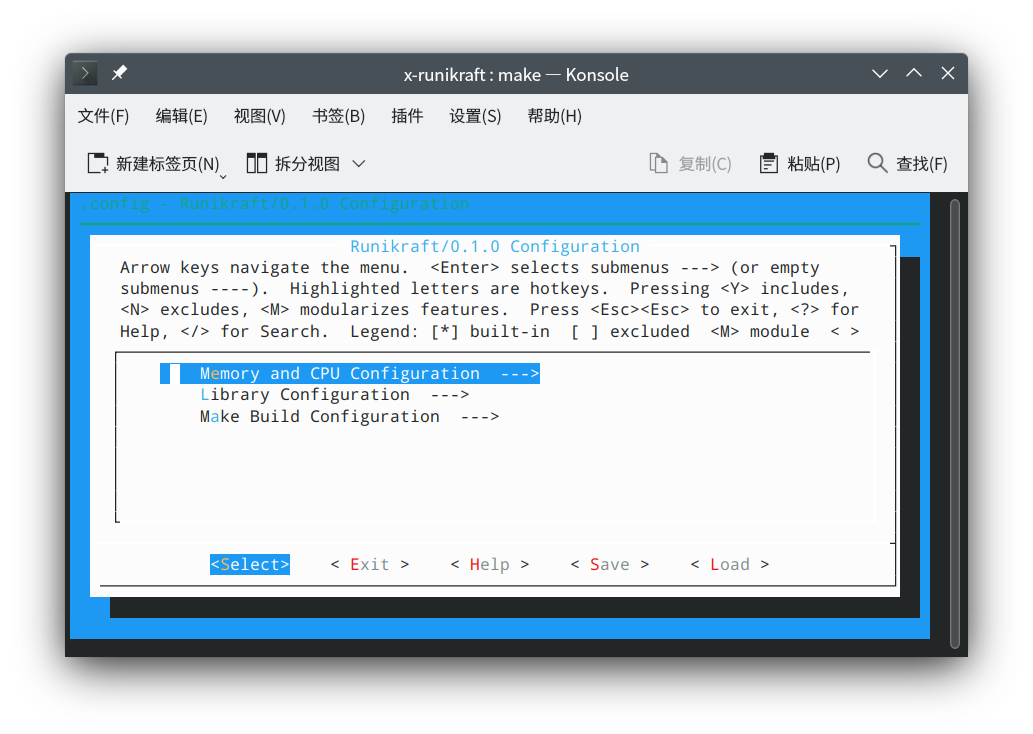
\includegraphics[width=0.8\linewidth]{assets/runikraft-menuconfig-1.png}
\caption{}
\label{fig:runikraft-menuconfig-1}
\end{figure}

配置系统并不是必不可少的,用户可以不使用menuconfig,直接修改\texttt{default\_config.rs}中的非bool
型编译参数,通过标准的cargo的.toml语法开启features。

\subsection{实现方法}

首先是\texttt{kconfig}的使用,我们参考了Chamberlain\cite{bib:kconfig}的使用方式,
在\texttt{support/scripts}中复用他的\texttt{build.Makefile}和\texttt{objects.Makefile},
并引入 submodule https://github.com/linux-kdevops/kconfig到\texttt{kconfig}文件夹,
然后在项目根目录下按照 kconfig 的语法编写对应的\texttt{Kconfig}文件:

\begin{lstlisting}
mainmenu "Runikraft/0.1.0 Configuration"

menu "Memory and CPU Configuration"
    config HEAP_SIZE
        int "Heap size(MiB)"
        default 16
    ...
    menu "Limit Configuration"
        ...
    endmenu

    ...
endmenu

menu "Library Configuration"
    source "lib/rkplat/config"
	source "lib/rkboot/config"
endmenu

...
endmenu
\end{lstlisting}

其中用\texttt{source "lib/@libname@/config"}引入相应模块中对应的配置菜单。
比如子模块\texttt{rkplat}的配置菜单如下图所示:

\begin{figure}[H]
\centering
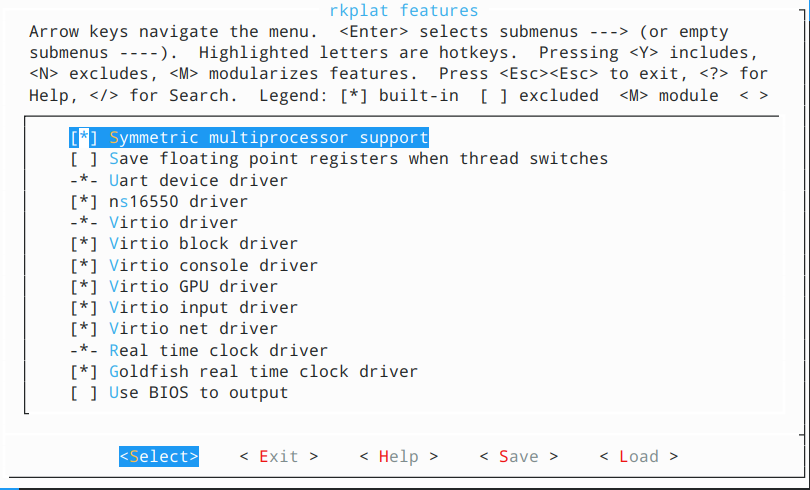
\includegraphics[width=0.7\linewidth]{assets/runikraft-menuconfig-2.png}
\caption{}
\label{fig:runikraft-menuconfig-2}
\end{figure}

这样我们最终的配置结果就会保存到项目根目录中的\texttt{.config}文件中。

在得到\texttt{.config}文件之后,接下来便要解决如何根据\texttt{.config}中的内容进行条件编译。
\texttt{menuconfig}生成的\texttt{.config}文件大致是下面这样:

\begin{lstlisting}[language={[gnu]make}]
#
# Memory and CPU Configuration
#
CONFIG_HEAP_SIZE=16
...

#
# Limit Configuration
#
CONFIG_MEMORY_SIZE=-1
CONFIG_OPEN_FILES=1024
...
# end of Limit Configuration
...
# end of Memory and CPU Configuration
...
\end{lstlisting}

这并不方便处理,因此我们只好采用一些不那么通用的方法来完成文件的读取和配置文件的输出。

上面已经提到,Runikraft 中是有两部分配置内容的,一部分是一些全局变量的数值,
另一部分是子模块中features的启用或禁用。

全局变量的默认数值存放在一个名为\texttt{default\_config.rs}的文件中,
我们需要根据\linebreak\texttt{.config}的内容来生成一个和\texttt{default\_config.rs}
的格式一样的文件\texttt{\$\{CONFIG\_DIR\}/\linebreak config.rs},然后再执行\texttt{cargo build}时传入环境变量\texttt{RUNIKRAFT\_CONFIG\_FILE=\linebreak"\$\{CONFIG\_DIR\}/config.rs"},
这样完成了全局变量数值的个性化配置。

features的启用使用的是\texttt{--features @featurename@}加在\texttt{cargo build}的
后面的方式(不加在后面默认禁用),于是我们需要根据\texttt{.config}的内容来生成类似于下面这样的一个字符串:

\begin{lstlisting}
--features rkplat/has_smp --features rkplat/driver_uart --features rkplat/driver_ns16550 --features rkplat/driver_virtio --features rkplat/driver_virtio_blk --features rkplat/driver_virtio_console --features rkplat/driver_virtio_gpu --features rkplat/driver_virtio_input --features rkplat/driver_virtio_net --features rkplat/driver_rtc --features rkplat/driver_goldfish_rtc --features rkboot/have_scheduler --features rkboot/sched_coop
\end{lstlisting}

这样就完成了子模块features的启用或禁用。

而上面的两项转换工作我们是用 C++ 程序来实现的。上面已经提到,menuconfig生成的\texttt{.config}文件并不方便处理,
因此我们的 C++ 程序采用的是不那么通用的方式来完成转换的,
详细代码位于\texttt{support/handle\_config.cpp}中,这里不再展示。

\section{总结}
经过两个月的不懈努力,我们最终实现了支持对称多处理器的抢占式的 RR 调度器、
密码学安全的随机数生成器、显示设备驱动、信号量原语、基于信箱的IPC等crates,
我们支持的设备有 ns16550、goldfish-rtc、virtio-blk、virtio-console、
virtio-rng、virtio-gpu、virtio-input、virtio-net。
我们还实现了基于 kconfig 的功能定制系统。尽管我们实现的功能与最初的设计仍有差距,但
已经足以用Runikraft写出有实用价值的程序了。为了展示 Runikraft,
我们写了基于 Runikraft 的数独程序(图\ \ref{fig:sudoku}),它拥有简单的图形界面,使用了 \texttt{rkallocbuddy}、\texttt{rkschedpreem}、\texttt{rklock}、\texttt{rkgpudev}等 crates,
能够比较全面地展示 Runikraft 的功能。在使用 release 配置构建时,数独程序的镜像大小只有 100KiB,由此
可见,引入图形界面不会显著增大镜像的大小,这对拓宽Unikernels的应用范围有积极意义。

\begin{figure}[tbh!]
\centering
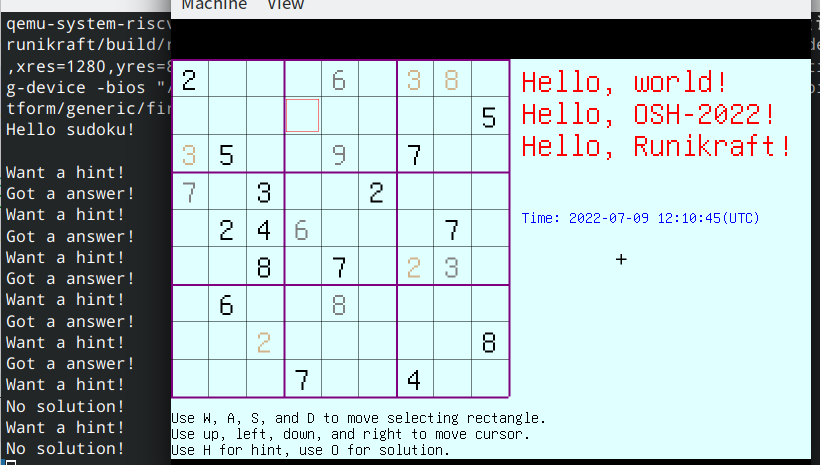
\includegraphics[width=0.6\linewidth]{assets/sudoku}
\caption{数独程序}
\label{fig:sudoku}
\end{figure}


Runikraft采用了全新的方式组织系统,系统由独立的crates组成,每个crate都可以独立发布和安装。
这对目前的自由操作系统的开发和发布有借鉴意义。

在Rust 1.59之前,内联汇编不能在stable channel的编译器中使用,使得用stable Rust写操作系统变得不可能。
在Rust 1.59发布后才开始开发的Runikraft是我们已知的唯一的
用stable Rust开发的操作系统。Runikraft的成功开发意味着用Rust写操作系统不再是试验性功能,
标志着Rust已经能胜任操作系统的开发。

\section{相关工作}

\subsection{安全容器}\sectionauthor{蓝俊玮}
《项目背景》中已指出,容器是云计算领域的常用的隔离手段,而由于容器并不是沙盒,
它提供的隔离能力不足以运行潜在的恶意代码,安全容器应运而生。从设计目标看,安全
容器的隔离能力与unikernels等同。安全容器的目标是能够直接运行ELF二进制文件,
而unikernels通常要求从源代码重新编译。

Kata Containers和gVisor都使用Go语言实现。

Kata Containers的实现思路是轻量级虚拟机,它是容器向uniKernel的过渡。它的主要特点是\cite{bib:kata}:
\begin{description}
\item[安全] Runs in a dedicated kernel, providing isolation of network,
I/O and memory and can utilize hardware-enforced isolation with virtualization VT extensions.
\item[兼容] Supports industry standards including OCI container format,
Kubernetes CRI interface, as well as legacy virtualization technologies.
\item[高效] Delivers consistent performance as standard Linux containers;
increased isolation without the performance tax of standard virtual machines.
\item[简洁] Eliminates the requirement for nesting containers inside full
blown virtual machines; standard interfaces make it easy to plug in and get started.
\end{description}

gVisor的实现思路是半虚拟化操作系统,它在用户空间运行,以拦截系统调用的方式为
应用程序提供服务。它与传统容器的关键区别是没有简单地将应用程序的系统调用重定向
给宿主机内核,而是实现了大多数内核原语,并基于这些原语实现系统调用。gVisor与unikernel的
区别是gVisor没有模拟硬件,而只是模拟了一个Linux内核;
unikernel本身是一个运行在虚拟硬件上的操作系统。
gVisor的特点:\cite{bib:gvisor}
\begin{description}
\item[容器原生安全] By providing each container with its own application kernel, gVisor limits the attack surface of the host. This protection does not limit functionality: gVisor runs unmodified binaries and integrates with container orchestration systems, such as Docker and Kubernetes, and supports features such as volumes and sidecars.

\item[资源高效] Containers are efficient because workloads of different shapes and sizes can be packed together by sharing host resources. gVisor uses host-native abstractions, such as threads and memory mappings, to co-operate with the host and enable the same resource model as native containers.

\item[跨平台] Modern infrastructure spans multiple cloud services and data centers, often with a mix of managed services and virtualized or traditional servers. The pluggable platform architecture of gVisor allows it to run anywhere, enabling consistent security policies across multiple environments without having to rearchitect your infrastructure.
\end{description}

\subsection{嵌入式系统}\sectionauthor{陈建绿}
大部分unikernels只打算在虚拟机上运行,但是IncludeOS和Rumprun支持在嵌入式设备上运行,
往年的ridiculous-includeos小组也做过将unikernel移植到嵌入式设备的研究。
可见嵌入式设备也是unikernel潜在的应用领域。嵌入式系统的类型丰富多样,这里着重介绍物联网(IoT)系统。

目前,物联网操作系统主要分为两大类,一是由传统的嵌入式实时操作系统(RTOS)发展而来,
比如FreeRTOS、LiteOS、RT-Thread;二是由互联网公司的云平台延伸而来,
基于传统操作系统进行“剪裁”和定制的IoT OS,比如Ali OS Things、TencentOS tiny、Win10 IOT。\cite{bib:iot-sys}

\href{https://github.com/OpenAtomFoundation/TencentOS-tiny}{TencentOS Tiny} 是腾讯
面向物联网领域开发的实时操作系统,具有低功耗,低资源占用,模块化,安全可靠等特点,
可有效提升物联网终端产品开发效率。

TencentOS tiny 提供精简的 RTOS 内核,内核组件可裁剪可配置,
可快速移植到多种主流 MCU (如 STM32 全系列)及模组芯片上。而且,
基于 RTOS 内核提供了丰富的物联网组件,内部集成主流物联网协议栈
(如CoAP/MQTT/TLS/DTLS/LoRaWAN/NB-IoT等),可助力物联网终端设备及
业务快速接入腾讯云物联网平台。

\href{https://github.com/ms-rtos}{MS-RTOS} (Micro Safe RTOS) 是翼辉信息全新设计的一款面向未来的
安全实时操作系统,其最大的特点是开创性地在没有 MMU 和资源受限的 MCU(如Cortex-M3)上也能支持多进程与动态装载技术,使得应用与系统能分离开发、独立升级;
MS-RTOS 支持内核空间内存保护(应用程序通过 syscall 访问内核),
使得内核有着非常高的安全性。MS-RTOS 在提供足够丰富功能的同时,保持了高效简洁的实现,
对 ROM、RAM 消耗极低,特别适用于对硬件成本敏感、安全性要求特别高的产品。\cite{bib:ms-rtos}

\begin{description}
\item[多进程] 允许运行多个进程,进程用户代码工作在 CPU 用户态,
通过系统调用(syscall)访问内核资源,利用 MPU 实现进程地址空间相互隔离。
\item[动态装载] 驱动与应用程序分离开发,应用与系统独立升级,
应用程序直接在 FLASH 中运行(无需加载到 RAM 执行,节约 RAM,运行速度更快)。
\item[内核安全] 进程用户代码工作在 CPU 用户态,通过系统调用
(syscall)进入内核, 保护内核不被进程破坏,利用 MPU 做到进程地址空间相互隔离,
进程影响范围最小化,掉电安全文件系统。
\end{description}
\subsection{用Rust编写的操作系统}
Rust语言的目标之一就是取代C语言,成为用于系统开发的底层语言。目前已有大量用Rust开发的操作系统:\cite{bib:rust-os-comparison}

\begin{longtable}{|>{\bfseries}l|p{0.11\linewidth}|p{0.02\linewidth}|p{0.02\linewidth}|p{0.08\linewidth}|p{0.06\linewidth}|p{0.02\linewidth}|p{0.02\linewidth}|p{0.05\linewidth}|p{0.08\linewidth}|p{0.08\linewidth}|}
\caption{用Rust实现的操作系统比较}\\
\hline
名称&\textbf{架构}&\textbf{纯} \rotatebox[origin=c]{-90}{\textbf{Rust}}&\textbf{活跃}&\textbf{内核架构}&\textbf{目标}&\textbf{用户态}&\rotatebox{-90}{\textbf{GUI}}&\textbf{贡献者数}&\textbf{文件系统}&\textbf{许可}\\\hline
\endfirsthead
\hline
名称&\textbf{架构}&\textbf{纯} \rotatebox[origin=c]{-90}{\textbf{Rust}}&\textbf{活跃}&\textbf{内核架构}&\textbf{目标}&\textbf{用户态}&\rotatebox{-90}{\textbf{GUI}}&\textbf{贡献者数}&\textbf{文件系统}&\textbf{许可}\\\hline
\endhead
redox&x86-32\newline x86-64&是&是&微内核&通用&是&是&50&ZFS\newline RedoxFS&MIT\\\hline
Theseus OS&x86-64\newline ARM WIP&是&是&Safe-language SAS/SPL OS&通用+嵌入式&&是&25&Custom\newline FAT32&MIT\\\hline
Tock&Cortex M&&是&&&&否&40&&APL 2/\newline MIT\\\hline
intermezzOS&x86-64&否&是&?&PoC&否&否&18&无&APL 2/\newline MIT\\\hline
RustOS&x86-32&?&是&无&PoC&否&否&10&无&APL 2/\newline MIT\\\hline
rustboot&x86-32&?&否&无&PoC&否&否&8&无&MIT\\\hline
\end{longtable}

其中的Redox是一款功能完整的类UNIX操作系统,而不只是操作系统内核,它包含C标准库、
窗口管理器、浏览器、文本编辑器、图像查看器、终端模拟器等众多软件包。

\section*{许可协议}\markboth{许可协议}
本文档以知识共享署名 4.0 国际 (CC BY 4.0)许可证发布。

\vspace{2ex}
\noindent\textbf{\large 您可以自由地}:
\begin{description}
\item[共享] 在任何媒介以任何形式复制、发行本作品;
\item[演绎] 修改、转换或以本作品为基础进行创作
在任何用途下,甚至商业目的。
\end{description}

\vspace{2ex}
\noindent\textbf{\large 惟须遵守下列条件}:
\begin{description}
\item[署名] 您必须给出适当的署名,提供指向本许可协议的链接,
同时标明是否(对原始作品)作了修改。您可以用任何合理的方式来署名,
但是不得以任何方式暗示许可人为您或您的使用背书。
\item[没有附加限制] 您不得使用法律术语或者技术措施,从而限制其他人
做许可协议允许的事情。
\end{description}

\vspace{2ex}
\noindent\textbf{\large 声明}:

您不必因为公共领域的作品要素而遵守许可协议,或者您的使用被可适用的例外或限制所允许。

不提供担保。许可协议可能不会给与您意图使用的所必须的所有许可。
例如,其他权利比如形象权、隐私权或人格权可能限制您如何使用作品。

本许可证的全文位于:\\
\centerline{\url{https://creativecommons.org/licenses/by/4.0/legalcode.zh-Hans}}


\begin{thebibliography}{99}
\bibitem{bib:feasibility-7} Steve Klabink. \textit{The Rust Programming Language}[M]. The Rust Community, 2019.
\bibitem{bib:feasibility-3} 张汉东. \textit{故事:Rust在企业领域的应用}[Z/OL]. 知乎专栏, 2019 (20190404) [2022-07-09] \url{https://web.archive.org/web/20220709104447/https://zhuanlan.zhihu.com/p/61410107}
\bibitem{bib:feasibility-0} \textit{About RISC-V}[Z/OL]. RISC-V International, 2021. \url{https://riscv.org/about/}
\bibitem{bib:feasibility-2} admin. \textit{RISC-V开源指令集架构简介与应用前景分析}[Z/OL]. ScenSmart一站式智能制造平台, 2019 (20191102) [2022-04-15]. \url{http://www.scensmart.com/news/the-introduction-of-risc-v-and-application-prospect-analysis/}

\bibitem{bib:os-concept} Abraham Silberschatz, Peter B. Galvin and Greg Gagne.
\textit{操作系统概念}[M]. 郑扣根, 唐杰, 李善平\ 译. 北京: 机械工业出版社, 2021: 54-58.

\bibitem{bib:docker-security-selinux} Daniel J Walsh. \texttt{Are Docker containers really secure?}[Z/OL]. Opensource.com, 2014 (20140622) [2022-04-10]. \url{https://opensource.com/business/14/7/docker-security-selinux}

\bibitem{bib:unikernel}
\textit{Unikernels: Rethinking Cloud Infrastructure}[Z/OL].
@unikernel [2022-02-18]. \url{https://web.archive.org/web/20220218194213/http://unikernel.org/}

\bibitem{bib:unikraft} Simon Kuenzer, Vlad-Andrei Bădoiu, Hugo Lefeuvre, Sharan Santhanam,
Alexander Jung, Gaulthier Gain, Cyril Soldani, Costin Lupu, \c{S}tefan Teodorescu, Costi Răducanu,
Cristian Banu, Laurent Mathy, Răzvan Deaconescu, Costin Raiciu and Felipe Huici.
\textit{Unikraft: Fast, Specialized Unikernels the Easy Way}[J/OL]. EuroSys '21, 2021, April: 26–29
[2022-03-27]. \url{https://dl.acm.org/doi/10.1145/3447786.3456248} \texttt{doi:10.1145/3447786.3456248}.

\bibitem{bib:unikernel-secuirty} Spencer Michaels and Jeff Dileo. \textit{Assessing Unikernel Security
}[R/OL]. Version 1.0. NCC Group, 2019: 4-10 [2022-03-27].
\url{https://research.nccgroup.com/wp-content/uploads/2020/07/ncc_group-assessing_unikernel_security.pdf}

\bibitem{bib:3-why-rust-pop}
Jake Goulding. \textit{What is Rust and why is it so popular?}[Z/OL]. Stack Overflow Blog. 2020 (20200120) [2022-03-24]. \url{https://web.archive.org/web/20220324021421/https://stackoverflow.blog/2020/01/20/what-is-rust-and-why-is-it-so-popular/}
\bibitem{bib:4-rust-go-cmp} CharyGao. \textit{也许是最客观、全面的比较 Rust 与 Go:都想把 Rust 也学一下}[Z/OL]. 博客园. 2020 (20201207) [2022-03-29]. \url{https://web.archive.org/web/20220329090604/https://www.cnblogs.com/Chary/p/14097609.html}
\bibitem{bib:5-why-rust2} 黄光星. \textit{为什么要使用 Rust 语言?Rust 语言的优势在哪里?}[Z/OL].
2020 (20200513) [2022-03-29] \url{https://www.zhihu.com/question/393796866}
\bibitem{bib:6-why-rust-pop-2} Krzysztof Wróbel. \textit{Rust programming language - what is rust used for and why is so popular?}[Z/OL]. codilime, 2022 (20220325) [2022-03-25]. \url{https://codilime.com/blog/why-is-rust-programming-language-so-popular/}
\bibitem{bib:7-rust-by-num} Pavan Belagatti.[\textit{Rust by the Numbers: The Rust Programming Language in 2021}[Z/OL]. The New Stack. 2021 (20210512) [2022-03-25]. \url{https://thenewstack.io/rust-by-the-numbers-the-rust-programming-language-in-2021/}
\bibitem{bib:8-rust-compatibility} \textit{Rust By Example}[M/OL]. Compatibility [2022-03-26]. \url{https://web.archive.org/web/20220326130141/https://doc.rust-lang.org/rust-by-example/compatibility.html}

\bibitem{bib:riscv-support} Jeff Tranter. \textit{What is RISC-V and Why is it Important?}[Z/OL]. ICS. 2021 (20210512) [2022-03-27]. \url{https://www.ics.com/blog/what-risc-v-and-why-it-important}
\bibitem{bib:riscv-gcc} \textit{Using the GNU Compilers Collections (GCC)}[G/OL]. 2021: RISC-V Options [2022-03-27]. \url{https://gcc.gnu.org/onlinedocs/gcc-11.2.0/gcc/RISC-V-Options.html#RISC-V-Options}
\bibitem{bib:riscv-llvm} \textit{Clang command line argument reference: Clang 15.0.0git documentation}[G/OL]. 2022: RISCV [2022-03-27] \url{https://clang.llvm.org/docs/ClangCommandLineReference.html#riscv}
\bibitem{bib:riscv-linux} Drew Fustini. \textit{Linux on RISC-V
with Open Hardware}[Z/OL]. Embedded Linux Conference, 2020 [2022-03-27]. \url{https://elinux.org/images/3/3d/Linux_riscv_elce2020.pdf}
\bibitem{bib:riscv-debian} \textit{RISC-V}[G/OL]. Debian Wiki, 2022 (2022-03-24) [2022-03-27]. \url{https://wiki.debian.org/RISC-V?action=recall&rev=151}

\bibitem{bib:riscv-spec1} \textit{The RISC-V Instruction Set Manual
Volume I: Unprivileged ISA}[S/OL]. Editors Andrew Waterman and Krste Asanović. Version 2.1. RISC-V Foundation, 2019 (20191213) [2022-03-25]. \url{https://github.com/riscv/riscv-isa-manual/releases/download/Ratified-IMAFDQC/riscv-spec-20191213.pdf}
\bibitem{bib:riscv-spec2} \textit{The RISC-V Instruction Set Manual
Volume II: Privileged Architecture}[S/OL]. Editors Andrew Waterman, Krste Asanović and John Hauser.
Version 1.9.1. RISC-V International, 2021 (20211204) [2022-03-27]. \url{https://github.com/riscv/riscv-isa-manual/releases/download/Priv-v1.12/riscv-privileged-20211203.pdf}
\bibitem{bib:riscv-spec3} \textit{RISC-V Debug Support
}[S/OL]. Editors Ernie Edgar and Tim Newsome. Version 1.0.0-Stable. SiFive, Inc., 2022(20220209)[2022-03-27]. \url{https://github.com/riscv/riscv-debug-spec/raw/b659d7dc7f578e1a2a76f9e62a5eec0f2d80045c/riscv-debug-stable.pdf}
\bibitem{bib:riscv-spec4} \textit{RISC-V Processor Trace}[S/OL]. Gajinder Panesar and
Iain Robertson. Version 1.0. UltraSoC Technologies Ltd., 2020(20200320)[2022-03-27]. \url{https://github.com/riscv/riscv-trace-spec/raw/e372bd36abc1b72ccbff31494a73a862367cbb29/riscv-trace-spec.pdf}

\bibitem{bib:amd64-manual} \textit{AMD64 Architecture Programmer's Manual: Volumes 1-5}[S/OL]. Revision 4.04, Advanced Micro Devices, Inc., 2021 (202111) [2022-03-27]. \url{https://www.amd.com/system/files/TechDocs/40332.pdf}
\bibitem{bib:amd64-manual-intel} \textit{Intel\textsuperscript{®} 64 and IA-32 Architectures Software Developer’s Manual}[S/OL]. Order Number: 325462-076US, Intel Corporation, 2021 (202112) [2022-03-27]. \url{https://cdrdv2.intel.com/v1/dl/getContent/671200}

\bibitem{bib:armv8-reference} \textit{Arm\textsuperscript{®} Architecture Reference Manual
for A-profile architecture}[S/OL]. Version 21.0, Arm Limited, 2022 [2022-03-27]. \url{https://developer.arm.com/documentation/ddi0487/latest}

\bibitem{bib:12-clickos} Joao Martins, Mohamed Ahmed, Costin Raiciu, Vladimir Olteanu,
Michio Honda, Roberto Bifulco and Felipe Huici. \textit{ClickOS and the Art of Network Function Virtualization}[C/OL]. 11th USENIX Symposium on Networked Systems
Design and Implementation. Seattle: USENIX Association. 2014: 459-473[2022-03-22]. \url{http://cnp.neclab.eu/projects/clickos/clickos.pdf}
\bibitem{bib:13-clickos2} Joao Martins, Mohamed Ahmed, Costin Raiciu and Felipe Huici.
\textit{Enabling Fast, Dynamic Network Processing with ClickOS}[J/OL]. HotSDN'13, 2013, August: 67-72[2022-03-22]. \url{http://cnp.neclab.eu/projects/clickos/clickos-workshop.pdf}

\bibitem{bib:11-unikerel2} Anil Madhavapeddy and David J. Scott. \textit{Unikernels: Rise of the Virtual Library Operating System}[J/OL]. ACM Queue, 2014, 11 [2022-03-22].  \url{https://queue.acm.org/detail.cfm?id=2566628}

\bibitem{bib:9-includeos}  Bratterud et al. \textit{IncludeOS: A minimal, resource efficient unikernel for cloud systems}[G/OL]. Adrian Colyer, The morning paper: a random walk through Computer Science research. 2016 (20160222) [2022-03-22]. \url{https://blog.acolyer.org/2016/02/22/includeos}
\bibitem{bib:10-includeos2} Nur Hussein. \textit{IncludeOS: a unikernel for C++ applications}[Z/OL]. 2017 (20170725) [2022-03-22]. \url{https://lwn.net/Articles/728682/}

\bibitem{bib:14-rusty-hermit} \textit{RustyHermit - A Rust-based, lightweight unikernel}[G/OL]. rusty-hermit 0.3.10. [2022-03-25]. \url{https://docs.rs/crate/rusty-hermit/0.3.10}
%\bibitem{bib:15-rust-runtime} Jason 于航. \textit{Rust Runtime 与 ABI}[M/OL]. 知乎专栏, 2021 (20210509) [2022-03-25] \url{https://zhuanlan.zhihu.com/p/370897059}
%\bibitem{bib:16-rust-runtime2} \textit{The Rust runtime}[G/OL]. The Rust Reference. [2022-03-17].
%\url{https://web.archive.org/web/20220317124224/https://doc.rust-lang.org/reference/runtime.html}
\bibitem{bib:17-rusty-hermit2} @stlankes. \textit{The \texttt{RustyHermit} Unikernel}[Z/OL]. Rust OSDev. 2021 (20210122) [2022-03-25]. \url{https://rust-osdev.com/showcase/rusty-hermit/}

\bibitem{bib:18-intra-unikernel} Mincheol Sung and Pierre Olivier. \textit{Intra-Unikernel Isolation with Intel Memory Protection Keys}[C/OL]. 16th ACM SIGPLAN/SIGOPS International Conference on Virtual Execution Environments. Lausanne: Association for Computing Machinery, 2022. \texttt{doi:10.1145/3381052.3381326}.
\bibitem{bib:19-mpk} \textit{Memory Protection Keys}[G/OL]. The Linux Kernel, 5.17.0. [2022-03-18]. \url{https://web.archive.org/web/20220318143208/https://www.kernel.org/doc/html/latest/core-api/protection-keys.html}
%\bibitem{bib:20-linux-kernel} Huo的藏经阁. \textit{linux内核那些事之Memory protection keys(硬件原理)}[Z/OL]. CSDN博客. 2021 (20211119) [2022-03-25]. \url{https://blog.csdn.net/weixin_42730667/article/details/121386896}
\bibitem{bib:21-rump-kernel} Wikipedia Contributors. \textit{Rump kernel}[G/OL]. Wikipedia, 2021 (20210903) [2022-03-29]. \url{https://en.wikipedia.org/w/index.php?title=Rump_kernel&oldid=1042218732}
\bibitem{bib:22-xen} Antti Kantee. \textit{Xen on Rump Kernels and the Rumprun Unikernel}[Z/OL]. XenProject, 2015 (20150806) [2021-08-18].  \url{https://web.archive.org/web/20210818101601/https://xenproject.org/2015/08/06/on-rump-kernels-and-the-rumprun-unikernel/}

\bibitem{bib:23-mirageos} Mircea Cosbuc. \textit{All About Unikernels: Part 2, Two Different Approaches, MirageOS and Rumprun}[Z/OL]. Container Solutions, 2020 (20200125) [2022-01-27]. \url{https://web.archive.org/web/2021*/https://blog.container-solutions.com/all-about-unikernels-part-2-mirageos-and-rumprun}
\bibitem{bib:24-rumrun} Sebastian Wicki. \textit{The Rumprun Unikernel}[Z/OL]. pkgsrcCon, 2016
[2022-03-25]. \url{https://pkgsrc.org/pkgsrcCon/2016/rumprun.pdf}
\bibitem{bib:canary} Wikipedia contributors. \textit{Sentinel species}[G/OL]. Wikipedia, 2022 (20220319) [2022-03-24]. \url{https://en.wikipedia.org/w/index.php?title=Sentinel_species&oldid=1078038868}
\bibitem{bib:unikraft-secuirty} \textit{Unikraft's Inherent Security Benefits}[Z/OL]. Unikraft, 2022 [2022-03-29]. \url{https://web.archive.org/web/20220329100701/https://unikraft.org/docs/features/security/}
\bibitem{bib:rcore-os} Yu Chen and Yifan Wu. \textit{rCore Tutorial Book}[M/OL]. Version 3,
2022(20220102) [2022-03-27]. \url{https://rcore-os.github.io/rCore-Tutorial-Book-v3/chapter0/0intro.html}

\bibitem{bib:kata} \textit{Kata Containers - Open Source Container Runtime Software}[Z/OL].
Kata Containers, [2022-04-02]. \url{https://web.archive.org/web/20220402043101/https://katacontainers.io/}

\bibitem{bib:gvisor} \textit{gVisor}[Z/OL]. [2022-04-02]. \url{https://web.archive.org/web/20220402043121/https://gvisor.dev/}

\bibitem{bib:feasibility-1}  Paolo Bonzini. \textit{Main Page}[G/OL]. QEMU Wiki, 2020 (20200609) [2022-04-15]. \url{https://wiki.qemu.org/index.php?title=Main_Page&oldid=9546}
\bibitem{bib:feasibility-5} RISC-V Platform Specification Task Group. \textit{RISC-V Supervisor Binary Interface Specification}[S/OL]. GitHub, 2022 (20220322) [2022-04-15]. \url{https://github.com/riscv-non-isa/riscv-sbi-doc/releases/tag/v1.0.0}
\bibitem{bib:feasibility-6} \textit{OpenSBI Version 1.0}[CP/OL]. GitHub, 2021 (20211224) [2022-04-15]. \url{https://github.com/riscv-software-src/opensbi/releases/tag/v1.0}
\bibitem{bib:feasibility-8} 肖猛. \textit{图解 Rust 所有权与生命周期}[M/OL]. 高宪凤. Rust精选. 2021 [2022-04-15]. \url{https://rustmagazine.github.io/rust_magazine_2021/chapter_1/rust_ownership.html}
\bibitem{bib:feasibility-9} hardsinging. \textit{Rust线程安全编程分析}[Z/OL]. 知乎专栏, 2022 (20220312) [2022-07-09]. \url{https://web.archive.org/web/20220709105413/https://zhuanlan.zhihu.com/p/138394529}
\bibitem{bib:feasibility-a} 尹天宇. \textit{RISC-V特权等级与Linux内核的启动}[Z/OL]. 知乎专栏, 2020 (20200823) [2022-07-09]. \url{https://web.archive.org/web/20220709105606/https://zhuanlan.zhihu.com/p/164394603}
\bibitem{bib:feasibility-b} 辣椒油li. \textit{RISC-V基本介绍}[Z/OL]. CSDN, 2022 (20220122) [2022-03-29]. \url{https://web.archive.org/web/20220329183308/https://blog.csdn.net/lijianyi0219/article/details/122634356}
\bibitem{bib:feasibility-c} orangeQWJ. \textit{RISC-V 特权指令结构}[Z/OL]. 博客园, 2022 (20220219) [2022-07-09].  \url{https://web.archive.org/web/20220709110346/https://www.cnblogs.com/orangeQWJ/p/15912780.html}
\bibitem{bib:feasibility-d} shawn. \textit{闲聊RISC-V虚拟化(1)-CPU虚拟化}[Z/OL]. 知乎专栏, 2021 (20210908) [2022-07-09]. \url{https://web.archive.org/web/20220709110755/https://zhuanlan.zhihu.com/p/408197895}

\bibitem{bib:2-why-rust} @程序师视野. \textit{我们为什么要选择小众语言 Rust 来开发软件?}[Z/OL]. 程序师. [2017-06-26]. \url{https://web.archive.org/web/20170626061304/https://www.techug.com/post/why-we-choose-rust-to-dev.html}
\bibitem{bib:1-rust-lang} \textit{Rust Programming Language}[G/OL]. [2022-03-26]. \url{https://web.archive.org/web/20220326232949/https://www.rust-lang.org/}
\bibitem{bib:risc-v-manual} David Patterson and Andrew Waterman. \textit{RISC-V 手册: 一本开源指令集的指南}[S]. 勾凌睿, 黄成, 刘志刚译. 2018: 13-21

\bibitem{bib:feasibility-e} 樊金昊, 左顺, 宁雨亭, 黄业琦, 张俸铭 and 雷思琦. \textit{可行性报告}[R/OL]. GitHub, 2019 (20190409) [2022-04-15]. \url{https://github.com/OSH-2019/x-rust-freertos/blob/2182e559cf5dedb68d0bf028f21298421cbedbb0/docs/feasibility.md}
\bibitem{bib:qemu-virt} \textit{`virt' Generic Virtual Platform (virt)}[G/OL]. QEMU Documentaion, [2022-07-09]. \url{https://web.archive.org/web/20220709110415/https://www.qemu.org/docs/master/system/riscv/virt.html}
\bibitem{bib:qemu7} Marius Nestor. \textit{QEMU 7.0 Released with KVM Support for RISC-V, ARM and OpenRISC Improvements}[N/OL]. 9TO5LINUX, 2022 (20220419) [2022-04-20]. \url{https://web.archive.org/web/20220420092003/https://9to5linux.com/qemu-7-0-released-with-kvm-support-for-risc-v-arm-and-openrisc-improvements}
\bibitem{bib:buddy-C-1} Evan Wallace. \textit{Buddy Memory Allocator}[CP/OL]. GitHub, 2018 (20180212) [2022-07-08]. \url{https://github.com/evanw/buddy-malloc/tree/254531aa101806ee665166920bd4c70e88730eb1}
\bibitem{bib:buddy-C-2} Stanislav Paskalev and Yun Hsiao Wu. \textit{buddy\_alloc}[CP/OL]. GitHub, 2022 (20220102) [2022-07-08]. \url{https://github.com/spaskalev/buddy_alloc/tree/6d6581605ae1254db7cdbc5ee2140d35f0bbac7b}
\bibitem{bib:buddy-C-3} Jinzhou Zhang. \textit{buddy-system}[CP/OL]. GitHub, 2013 (20131211) [2022-07-08]. \url{https://github.com/lotabout/buddy-system/tree/21b9a8edce16ada9622e53c12d4a2a23b92f5749}
\bibitem{bib:buddy-Rust-1} jiegec, Vinay Chandra, Runji Wang, Luo Jia, Richard Chien and
Tom Dohrmann. \textit{buddy\_system\_allocator}[CP/OL]. GitHub, 2022 (20220605) [2022-07-08]. \url{https://github.com/rcore-os/buddy_system_allocator/tree/72c01c53eca8fac39fde29842523ec9d3d965929}
\bibitem{bib:buddy-Rust-2} ARaspiK. \textit{Buddies: A low-level buddy allocator}[CP/OL]. GitHub, 2019 (20190514) [2022-07-08]. \url{https://github.com/araspik/buddies/tree/f607d4c015c0c2bd2ab069a7413045ffdd440b39}
\bibitem{bib:buddy-Rust-3} Eric Kidd and Jethro Beekman. \textit{\texttt{alloc\_buddy\_simple}: A simple ``buddy allocator'' for bare-metal Rust}[CP/OL]. 2016 (20160919) [2022-07-08]. \url{https://github.com/emk/toyos-rs/tree/b29fda8cab38ee51945bd73174ece15481409941/crates/alloc_buddy_simple}
\bibitem{bib:rust-test} 繁星点点尽在你的指尖. \textit{单元测试、集成测试}[G/OL].
Rust语言圣经(Rust Course), 2022 [2022-07-02]. \url{https://web.archive.org/web/20220702105534/https://course.rs/test/unit-integration-test.html}
\bibitem{bib:kconfig} Luis Chamberlain. \texttt{Adapting Linux kernel kconfig}[CP/OL]. GitHub, 2022 (20220205) [2022-07-01]. \url{https://github.com/mcgrof/init-kconfig/tree/325fc60d21384742d137f9ea5bf66b2478021bce}

\bibitem{bib:iot-sys} 刘于苇. \textit{与嵌入式RTOS大不同,主流物联网操作系统中哪款适合你?}[Z/OL].
电子工程专辑, 2021 (20210518) [2022-03-12]. \url{https://www.eet-china.com/news/202105180818.html}
\bibitem{bib:ms-rtos} ScilogyHunter. \textit{MS-RTOS正式发布啦!!!}[Z/OL]. CSDN, 2020 (20200716) [2022-03-12]. \url{https://blog.csdn.net/ScilogyHunter/article/details/107390947}
\bibitem{bib:rust-os-comparison} flosse, wmanley, ticki, et al. \textit{Rust OS comparison}[G/OL]. GitHub, 2022 (20220408) [2022-04-10]. \url{https://github.com/flosse/rust-os-comparison/tree/f3eb1aae4f080fafd81b44254f54e387ac5f6b9d}
\end{thebibliography}
\end{document}
